\documentclass{beamer}
\usepackage[english]{babel}
\usepackage{color}
\usepackage{hyperref}
\usepackage{graphicx}
\usepackage{multibbl}
\usepackage[utf8x]{inputenc}
\usepackage[version=3]{mhchem}
\usepackage{amsmath}
\usepackage{amssymb}
\usepackage{amsfonts}
\usepackage{amsopn}
\usepackage{braket}
\usepackage{bbm}
\usepackage{dsfont}
\usepackage{kpfonts}
% \usepackage{mathabx}

\parindent=0cm


% Various new commands that ease typesetting math even further
% \newcommand{\assign}{\ensuremath{\coloneq}}
% \newcommand{\rassign}{\ensuremath{\eqcolon}}
\newcommand{\assign}{\ensuremath{:=}}
\newcommand{\rassign}{\ensuremath{=:}}

\newcommand{\of}[1]{\ensuremath{\left( #1 \right)}}
\newcommand{\ofs}[1]{\ensuremath{\left( #1 \right)}}

\newcommand{\norm}[1]{\ensuremath{\| #1 \|}}

\newcommand{\tmop}[1]{\ensuremath{\operatorname{#1}}}

\newcommand{\id}{\ensuremath{\mathds{1}}}
% \newcommand{\id}{\ensuremath{I}}


\newcommand{\conj}[1]{\ensuremath{\overline{#1}}}

\newcommand{\T}{\ensuremath{{}^{\textnormal{T}}}}
\newcommand{\herm}{\ensuremath{{}^{\textnormal{H}}}}

\newcommand{\ft}[1]{\ensuremath{\mathcal{F}\left(#1\right)}}
\newcommand{\ift}[1]{\ensuremath{\mathcal{F}^{-1}\left(#1\right)}}

\newcommand{\fft}[1]{\ensuremath{\mathtt{FFT}\left(#1\right)}}
\newcommand{\ifft}[1]{\ensuremath{\mathtt{IFFT}\left(#1\right)}}

\newcommand{\dotp}[2]{\ensuremath{\langle #1 , #2 \rangle}}

\newcommand{\bigO}[1]{\ensuremath{\mathcal{O}\left( #1 \right)}}

\newcommand{\mat}[1]{\ensuremath{\mathbf{#1}}}

% multi-indices
\newcommand{\mindex}[1]{\ensuremath{\underline{#1}}}

\newcommand{\laplace}{\ensuremath{\operatorname{\Delta}}}

% EOF


\mode<presentation>
{
  \usetheme{Montpellier}
  \setbeamercovered{transparent}
}

\synctex=1
\parindent 0pt

\title[Numerical Steepest Descent for Hagedorn Wavepackets]
      {Numerical Steepest Descent \\
       for Overlap Integrals \\
       of Hagedorn Wavepackets}
\author[]{Raoul Bourquin}

\date{Disentis 2014}


\newbibliography{nsd}
\newbibliography{hawp}
\newbibliography{sqs}
\newbibliography{sdwp}
\newbibliography{chem}

\beamertemplatenavigationsymbolsempty

\newcommand{\cemph}[1]{\emph{\color{orange} #1}}
% -----------------------------------------------------------------------------------------
\begin{document}

\begin{frame}
  \titlepage
\end{frame}

\begin{frame}{Outline}
  \tableofcontents
\end{frame}


\section{Motivation}
\begin{frame}{Motivation}
  \begin{itemize}
    \item Simulation of Photoionization of \ce{Hg2}
    \begin{itemize}
      \item Initial value $\ket{\Psi_0}$
      \item Time-propagated value $\ket{\Psi_t}$
    \end{itemize}
  \end{itemize}
  \begin{figure}
    \centering
    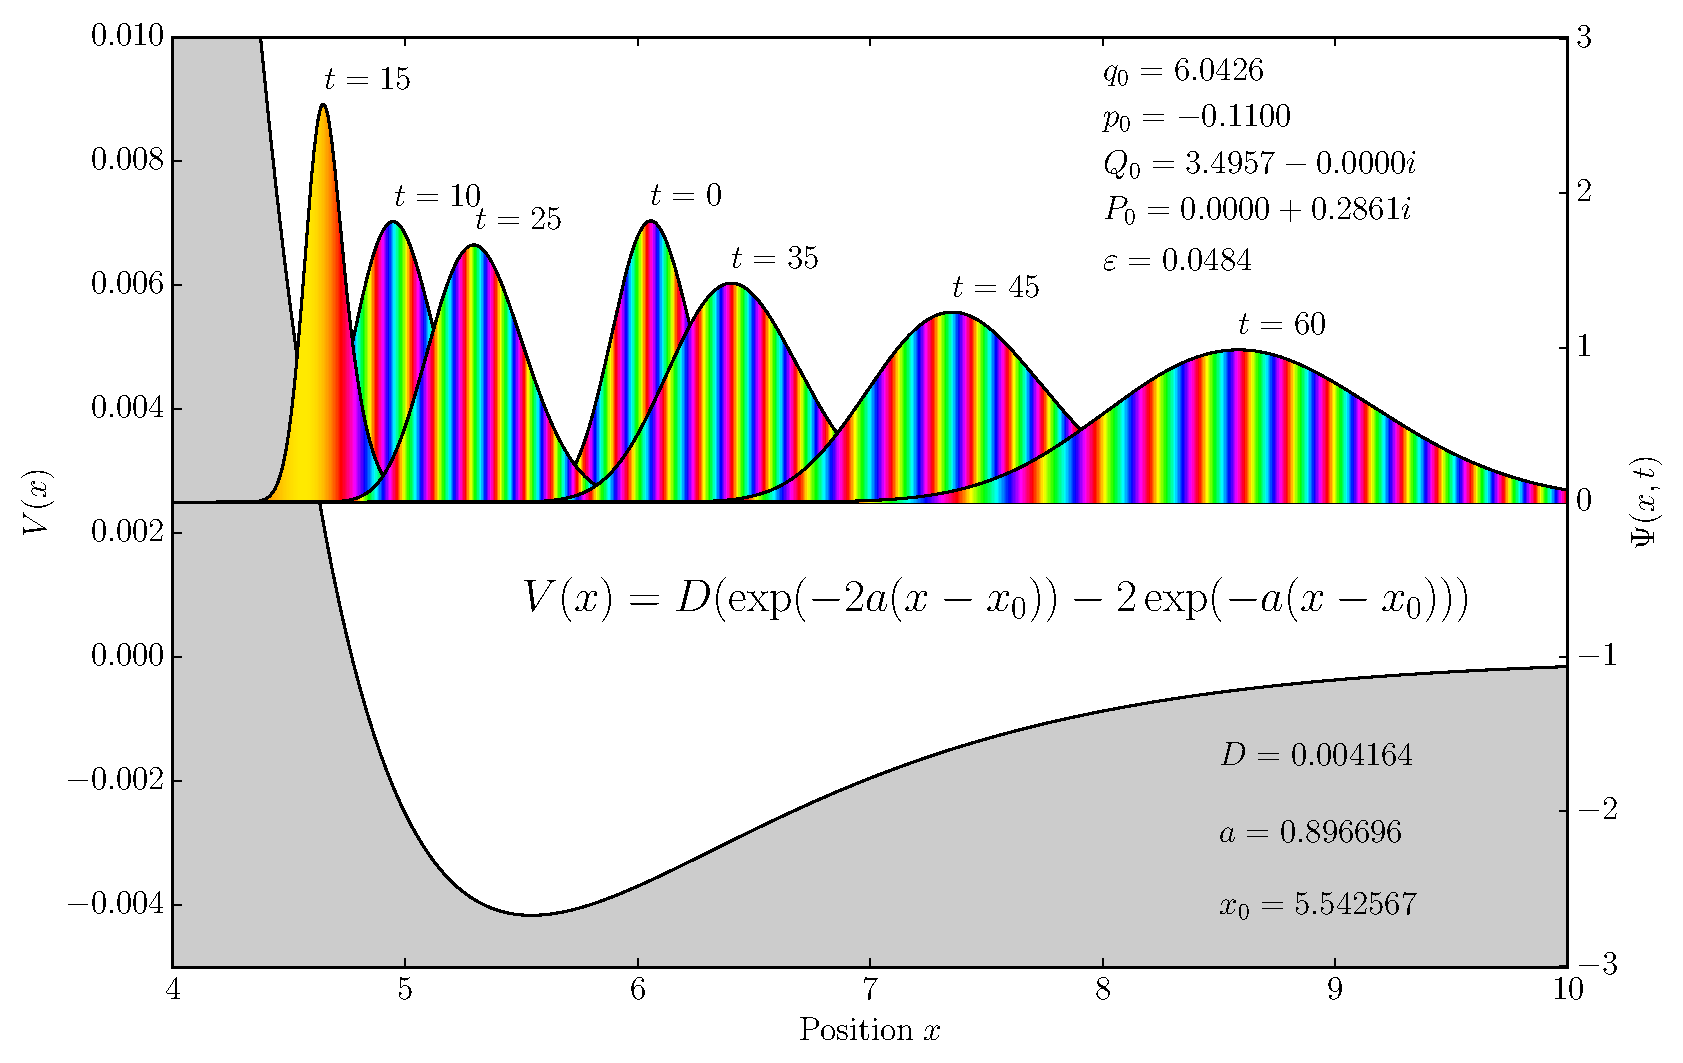
\includegraphics[width=0.6\linewidth]{./fig/hg_morse_wps.pdf}
  \end{figure}
  \nocite{chem}{SIZ_hg2}
  \tiny
  \bibliographystyle{chem}{abbrv}
  \bibliography{chem}{chem}{}
\end{frame}


\begin{frame}{Motivation}
  \begin{itemize}
    \item Compute autocorrelation $|A(t)|$
    \begin{equation*}
      A(t) \assign \Braket{\Psi_0 | \Psi_t}
           = \idotsint_{\mathbb{R}^D} \conj{\Psi_0(\vec{x})} \Psi_t(\vec{x}) \di{\vec{x}}
    \end{equation*}
    \item Common techniques give \cemph{wrong} results
  \end{itemize}
  \begin{figure}
    \centering
    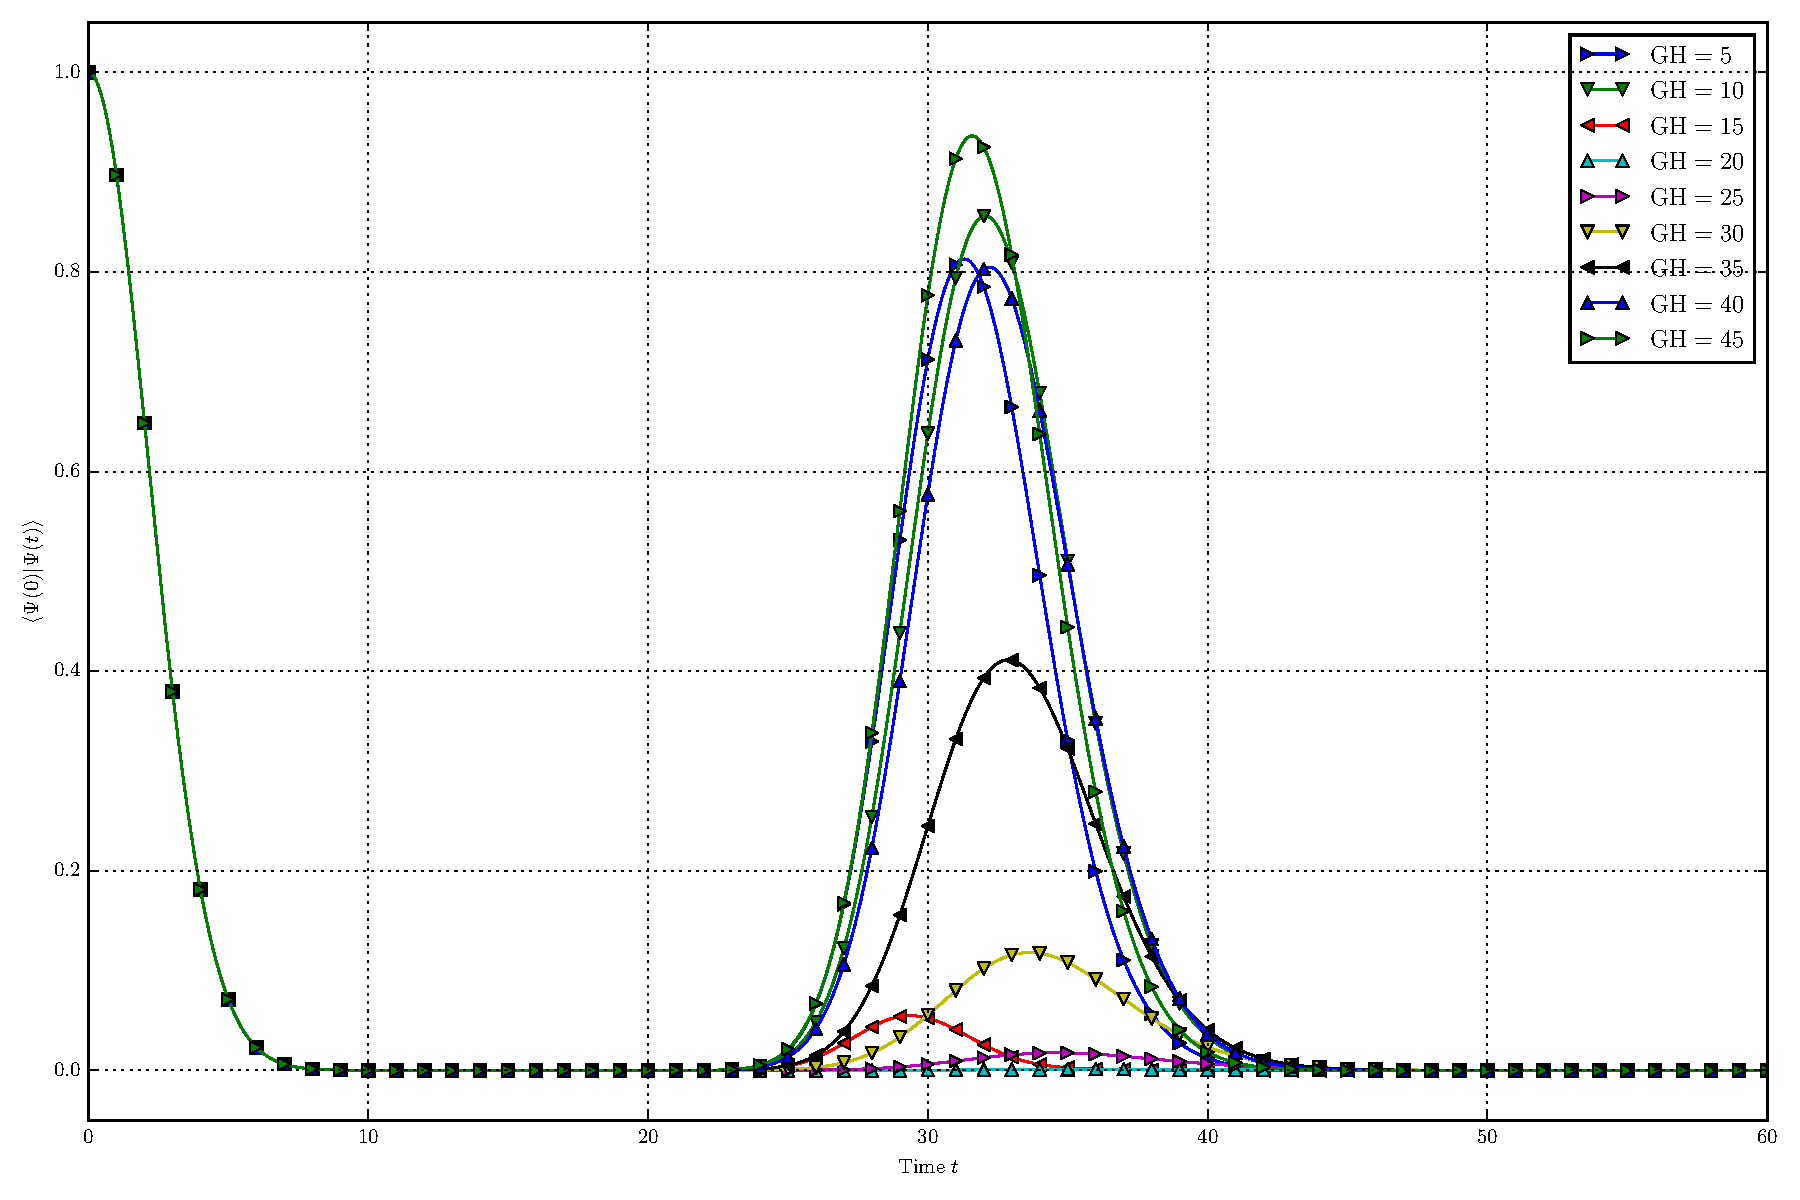
\includegraphics[width=0.6\linewidth]{./fig/ac_mercurial_morse.pdf}
  \end{figure}
\end{frame}


\section{Highly Oscillatory Integrals}


\begin{frame}{Highly Oscillatory Integrals}{Typical Example}
  \begin{minipage}{0.5\linewidth}
    \begin{equation*}
      I = \int_{\Omega} f(\vec{x}) e^{\imath \omega g(\vec{x})} \di{\vec{x}}
    \end{equation*}
    \begin{itemize}
      \item Oscillator $g(\vec{x})$ (non-oscillatory)
      \item Envelope $f(\vec{x})$ (non-oscillatory)
      \item Frequency $\omega \in \mathbb{R}^{+}$
      \item Domain $\Omega \subseteq \mathbb{R}^D$
    \end{itemize}
  \end{minipage}
  \begin{minipage}{0.48\linewidth}
    \begin{figure}
      \centering
      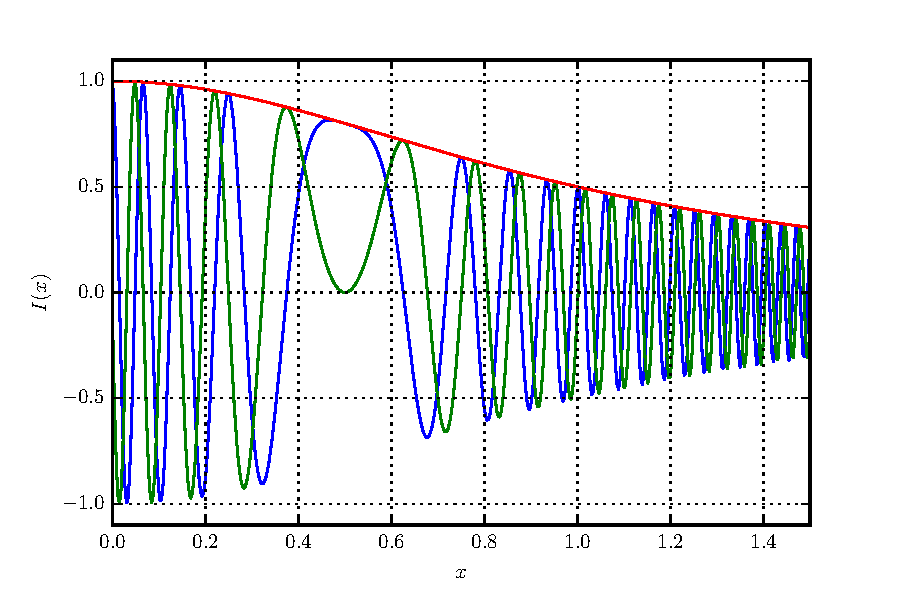
\includegraphics[width=\linewidth]{./fig/oscillatory_example.pdf}
    \end{figure}
    \vspace{-0.6cm}
    \begin{align*}
      f(x) & = \frac{1}{1+x^2} \\
      g(x) & = \left(x - \frac{1}{2}\right)^2 \\
      \omega & = 100
    \end{align*}
  \end{minipage}
\end{frame}


\begin{frame}{Highly Oscillatory Integrals}{Typical Example}
  \begin{minipage}{0.5\linewidth}
    Compute:
    \begin{equation*}
      \int_{-2}^3 \int_{-2}^3 \frac{e^{5 \imath \left(x^2-x y-y^2\right)}}{1 + (x+y)^2} \di{x} \di{y}
    \end{equation*}
    where:
    \begin{align*}
      f(x) & = \frac{1}{1 + (x+y)^2} \\
      g(x) & = x^2 - x y - y^2 \\
    \end{align*}
    and $\omega = 5$
  \end{minipage}
  \begin{minipage}{0.48\linewidth}
    \begin{figure}
      \centering
      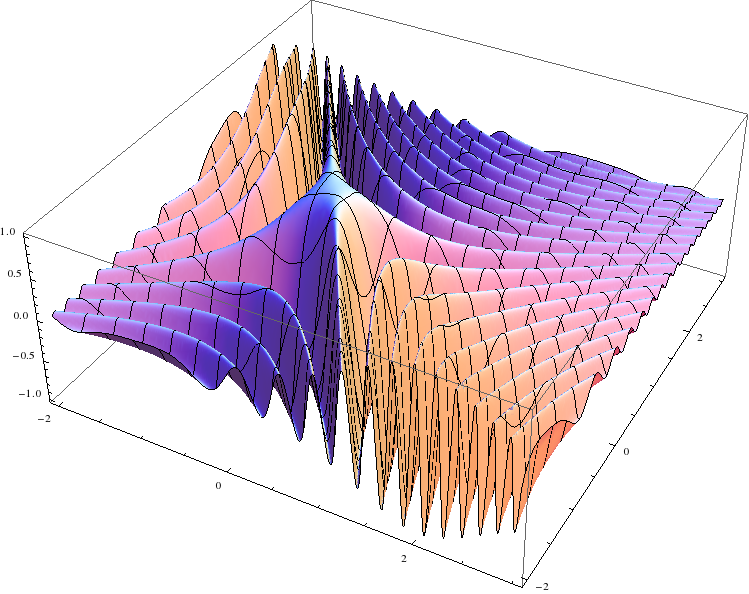
\includegraphics[width=\linewidth]{./fig/oscillatory_example_2d.png}
    \end{figure}
  \end{minipage}
\end{frame}


\section{The Numerical Steepest Descent Method}


\begin{frame}{Numerical Steepest Descent}{Central Observations}
  Oscillatory part $e^{\imath \omega g(x)}$ of:
  \begin{equation*}
    I = \int_a^b f(x) e^{\imath \omega g(x)} \di{x}
  \end{equation*}
  does:
  \begin{itemize}
    \item decay exponentially fast for increasing $\Im g(z)$
    \item not oscillate for constant $\Re g(z)$
  \end{itemize}
  because:
  \begin{equation*}
    e^{\imath \omega g(z)}
    =
    e^{\imath \omega (\Re g(z) + \imath \Im g(z))}
    =
    e^{\imath \omega \Re g(z)}
    e^{- \omega \Im g(z)}
  \end{equation*}
\end{frame}


\begin{frame}{Numerical Steepest Descent}{Main Idea and Overview}
  \begin{itemize}
    \item Transform the integrand such that it is no longer oscillatory but rather exponentially decaying.
  \end{itemize}
  \vspace{1cm}
  \begin{itemize}
    \item Find a coordinate transformation $z = h(\tau)$ such that the \cemph{real} part
          of $g(z)$ is constant.
    \item Apply Cauchy's Theorem for contour integrals along $h(\tau)$.
  \end{itemize}
\end{frame}


\begin{frame}{Numerical Steepest Descent}{Contributions to the Integral}
  \begin{minipage}{0.6\linewidth}
    Which parts do contribute?
    \begin{itemize}
      \item Endpoints of the interval: $[a, b]$
      \item \cemph{stationary points}: $\nabla g(\vec{x}) = \vec{0}$
      \item \cemph{resonance points}: $\nabla g(\vec{x}) \perp \partial \Omega$
    \end{itemize}
  \end{minipage}
  \begin{minipage}{0.38\linewidth}
    \begin{figure}
      \centering
      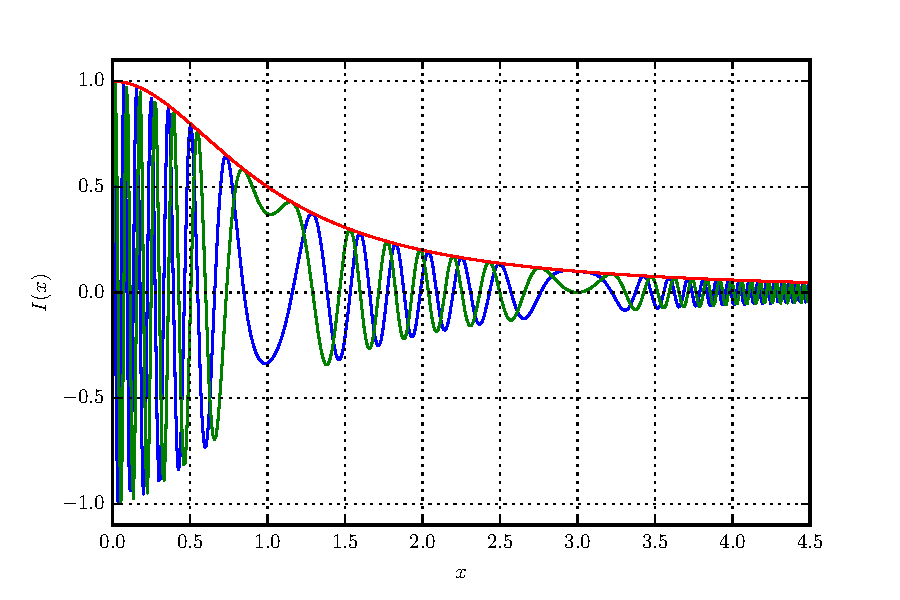
\includegraphics[width=\linewidth]{./fig/oscillatory_example_2.pdf}
    \end{figure}
  \end{minipage}
  Intuitive explanation:
  \begin{itemize}
    \item Oscillations in integrand generally cancel
    \item Places with locally no oscillations contribute
  \end{itemize}
\end{frame}


\begin{frame}{Numerical Steepest Descent}{The Path Equation}
  \begin{minipage}{0.58\linewidth}
    \begin{itemize}
      \item Set of contributing points:
      \begin{equation*}
        \Theta := \{a, b\} \cup \{x^{*}_j\}_j
      \end{equation*}
    \end{itemize}
    \begin{itemize}
      \item Path equations:
      \begin{itemize}
        \item $\forall \xi \in \Theta$:
        \begin{equation*}
          g(h_\xi(\tau)) = g(\xi) + \imath \tau
        \end{equation*}
        \item yields path $h_{\xi}(\tau)$ with $\tau \in \mathbb{R}_0^{+}$
      \end{itemize}
    \end{itemize}
  \end{minipage}
  \begin{minipage}{0.40\linewidth}
    \begin{figure}
      \centering
      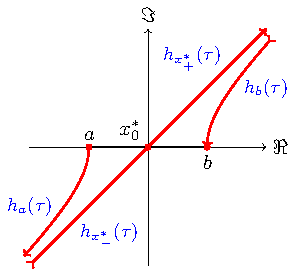
\includegraphics[width=\linewidth]{./fig/nsd_path_figure.pdf}
    \end{figure}
  \end{minipage}
\end{frame}


\begin{frame}{Numerical Steepest Descent}{Solving the Path Equation}
  \begin{minipage}{0.58\linewidth}
    \begin{itemize}
      \item Inverse of $g$ possibly multivalued
      \item Endpoints:
        \begin{itemize}
          \item compute $h_a$ and $h_b$
          \item choose by conditions:
          \begin{equation*}
            h_a(0) = a, \quad h_b(0) = b
          \end{equation*}
        \end{itemize}
      \item Stationary points:
        \begin{itemize}
          \item choose two $h_{x^{*}_j,+}$ and $h_{x^{*}_j,-}$
          \item paths lead to the same \cemph{valley}
        \end{itemize}
        % TODO: Go into more details?
    \end{itemize}
  \end{minipage}
  \begin{minipage}{0.40\linewidth}
    \begin{figure}
      \centering
      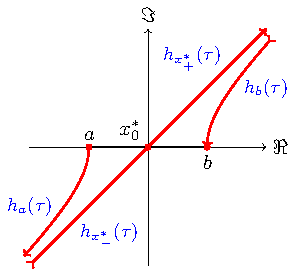
\includegraphics[width=\linewidth]{./fig/nsd_path_figure.pdf}
    \end{figure}
  \end{minipage}
\end{frame}


\begin{frame}{Numerical Steepest Descent}{Assemble the Parts}
  \begin{itemize}
    \item Perform transformations $x \mapsto h_{\xi}(\tau)$
    \begin{equation*}
      J[\xi] :=
      e^{\imath \omega g(\xi)}
      \int_{0}^{\infty}
        f(h_{\xi}(\tau)) \,
        h_{\xi}^{\prime}(\tau) \,
        e^{-\omega \tau} \,
      \mathrm{d}\tau
    \end{equation*}
    \item Apply Cauchy's Theorem
    \begin{equation*}
      I = e^{\imath\omega g(a)} J[a]
        + \sum_{j} \left(J[x_{j,+}^{*}] - J[x_{j,-}^{*}]\right)
        - e^{\imath\omega g(b)} J[b]
    \end{equation*}
    \item Restrictions: poles and branch cuts
    \item Just transformation of the problem
  \end{itemize}
\end{frame}


\begin{frame}{Numerical Steepest Descent}{Quadrature}
  \begin{itemize}
    \item New problem to compute:
    \begin{equation*}
      J[\xi] :=
      e^{\imath \omega g(\xi)}
      \int_{0}^{\infty}
        f(h_{\xi}(\tau)) \,
        h_{\xi}^{\prime}(\tau) \,
        e^{-\omega \tau} \,
      \mathrm{d}\tau
    \end{equation*}
    \item (Generalized) Gauss-Laguerre quadrature $\{\gamma_k, w_k\}_{k=1}^K$
    \begin{equation*}
    J[\xi] \approx
    \frac{e^{\imath \omega g(\xi)}}{\omega}
    \sum_{k=1}^K
      f\left(h_{\xi}\left(\frac{\gamma_k}{\omega}\right)\right)
      h_{\xi}^{\prime}\left(\frac{\gamma_k}{\omega}\right)
      w_k
    \end{equation*}
    %\item Number of integrals can grow exponentially
    \item Integrals (weakly) singular
    \item There can be many paths
  \end{itemize}
\end{frame}


\begin{frame}{Numerical Steepest Descent}{Main Decomposition Theorem}
  \begin{theorem}[Huybrechs and Vandewalle, 2006]
    Assume that the functions $f$ and $g$ are analytic in a simply connected and
    sufficiently (infinitely) large complex region $D$ containing the interval $[a, b]$.
    Assume further that the equation $g(x) = 0$ has only one solution $x^{*}$ in $D$ and
    $x^{*} \in (a, b)$. Define $g_1 \assign g|_{[a,x^{*}]}$ and $g_2\assign g|_{[x^{*},b]}$.
    If the following conditions hold:
    \begin{align*}
      \exists m \in \mathbb{N} : |f(z)| & = \mathcal{O}(|z|^m), \\
      \exists \omega_0 \in \mathbb{R} : |g_1^{-1}(z)| & = \mathcal{O}(e^{\omega_0 |z|}) \\
                                        |g_2^{-1}(z)| & = \mathcal{O}(e^{\omega_0 |z|})
    \end{align*}
    as $|z| \rightarrow \infty$ then
  \end{theorem}
\end{frame}


\begin{frame}{Numerical Steepest Descent}{Main Decomposition Theorem, continued}
  \begin{theorem}[Huybrechs and Vandewalle, 2006]
    there exist functions $F_j(\xi), j = 1, 2$ of the form:
    \begin{equation*}
      F_j(\xi) \assign \int_{\Gamma_{\xi,j}} f(z) e^{\imath \omega g(z)} \di{z}
    \end{equation*}
    with $\Gamma_{\xi,j}$ a path that starts at $\xi$, such that:
    \begin{equation*}
      \int_s^t f(z) e^{\imath \omega g(z)} \di{z} =
      F_1(s) - F_1(x^{*}) + F_2(x^{*}) - F_2(t), \quad \forall \omega > (m+1)\omega_0,
    \end{equation*}
    for $s \in [a, x^{*}]$ and $t \in [x^{*}, b]$. A parameterization
    $h_{\xi,j}(\tau)$, $\tau \in [0, \infty)$, for $\Gamma_{\xi,j}$ exists such that
    the integrand of $F_{j}$ is $\mathcal{O}(e^{−\omega \tau})$.
  \end{theorem}
\end{frame}


\begin{frame}{Numerical Steepest Descent}{Extensions and Outlook}
  This was for closed intervals. What about:
  \vspace{0.2cm}
  \begin{itemize}
    \item semi-infinite intervals $[a, \infty)$?
    \begin{itemize}
      \item works the same (no correct proof yet)
    \end{itemize}
    \item infinite intervals $(-\infty, \infty)$?
    \begin{itemize}
      \item decompose into two semi-infinite intervals
    \end{itemize}
    \item multiple stationary points?
    \begin{itemize}
      \item apply procedure at each $x^{*}_i$
    \end{itemize}
    \item complex stationary points $x^{*} \in \mathbb{C} \setminus \mathbb{R}$?
    \begin{itemize}
      \item put path through the point
    \end{itemize}
    \item higher dimensions?
    \begin{itemize}
      \item much more involved and complicated theory
    \end{itemize}
  \end{itemize}
\end{frame}


\begin{frame}{Numerical Steepest Descent}{Example $g(x) := x^2$}
  \vspace{-0.5cm}
  \begin{equation*}
    I = \int_{-1}^{1} 1\, e^{\imath \omega x^2} \di{x}
    \quad \text{with} \quad
    g(x) \assign x^2
  \end{equation*}
  \begin{equation*}
    g^{\prime}(x) = 0 \quad \Rightarrow \quad x^{*} = 0
  \end{equation*}
  \begin{equation*}
    \begin{split}
    g(h_{-1}) = g(-1) + \imath \tau   & \Rightarrow
    h_{-1}(\tau) = -\sqrt{1+\imath\tau}, \quad
    h_{-1}^{\prime}(\tau) = -\frac{\imath}{2\sqrt{1+\imath\tau}} \\
    g(h_{1}) = g(1) + \imath \tau   & \Rightarrow
    h_{1}(\tau) = \sqrt{1+\imath\tau}, \quad
    h_{1}^{\prime}(\tau) = \frac{\imath}{2\sqrt{1+\imath\tau}} \\
    g(h_{0}) = g(0) + \imath \tau   & \Rightarrow
    h_{0,\pm}(\tau) = \pm\sqrt{\imath\tau}, \quad
    h_{0,\pm}^{\prime}(\tau) = \pm\frac{\imath}{2\sqrt{\tau}}
    \end{split}
  \end{equation*}
  \begin{equation*}
    \begin{split}
%     I = e^{\imath\omega} \int_0^\infty h_{-1}^{\prime}(\tau) e^{-\omega\tau} \di{\tau}
%     - \int_0^\infty h_{0,-}^{\prime}(\tau) e^{-\omega\tau} \di{\tau} \\
%     + \int_0^\infty h_{0,+}^{\prime}(\tau) e^{+\omega\tau} \di{\tau}
%     - e^{\imath\omega} \int_0^\infty h_{1}^{\prime}(\tau) e^{-\omega\tau} \di{\tau}
      I = e^{\imath\omega} \int_0^\infty -\frac{\imath e^{-\omega\tau}}{2\sqrt{1+\imath\tau}} \di{\tau}
      - \int_0^\infty -\frac{\imath e^{-\omega\tau}}{2\sqrt{\tau}} \di{\tau} \\
      + \int_0^\infty  \frac{\imath e^{-\omega\tau}}{2\sqrt{\tau}} \di{\tau}
    - e^{\imath\omega} \int_0^\infty \frac{\imath e^{-\omega\tau}}{2\sqrt{1+\imath\tau}} \di{\tau}
    \end{split}
  \end{equation*}
\end{frame}


\begin{frame}{Numerical Steepest Descent}{Complex Stationary Points}
  \vspace{-0.5cm}
  \begin{equation*}
    \int_{-2}^{2} \log\left(2+x^2\right) e^{50 \imath \left(\delta x + \frac{x^3}{3}\right)} \di{x}
  \end{equation*}
  with $\delta \in \{10, 5, 2, 1, \frac{1}{2}, \frac{1}{5}, \frac{1}{10}, \frac{1}{100}, 0\}$
  and $x^{*} = \imath \sqrt{\delta}$
  \begin{figure}
    \centering
    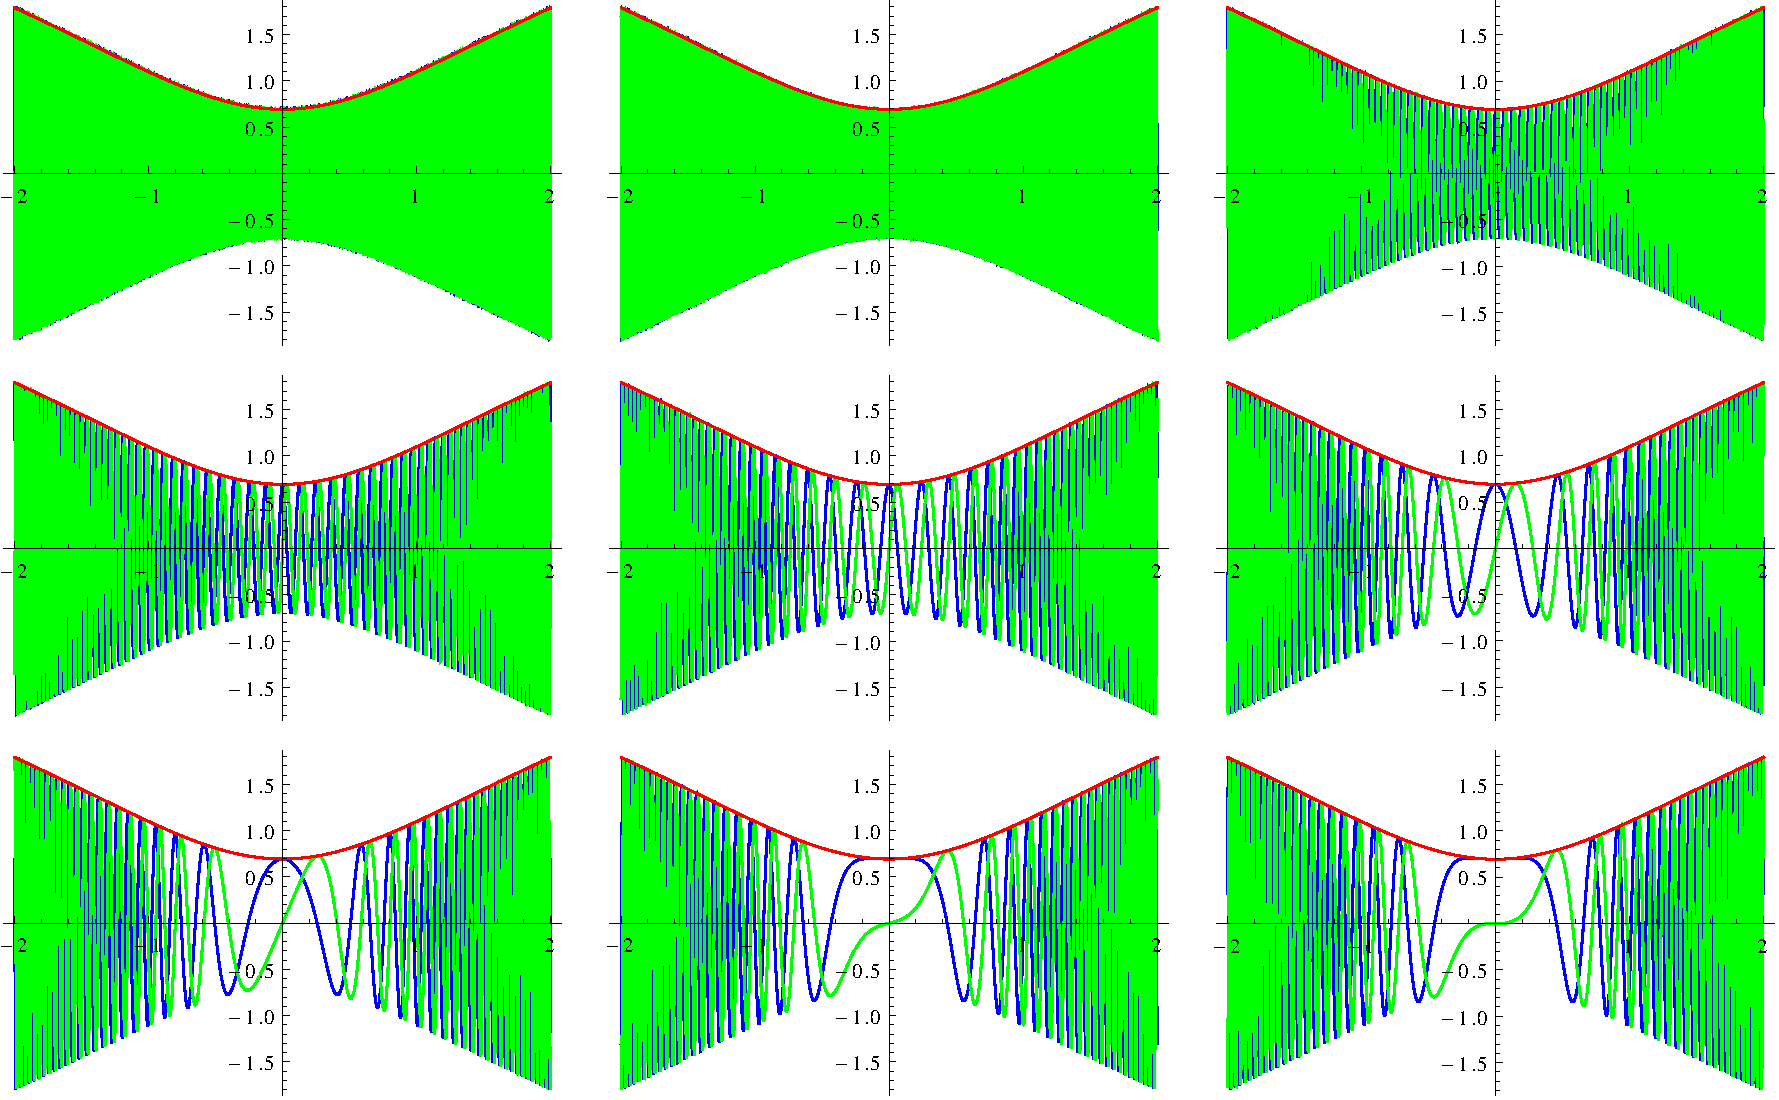
\includegraphics[width=0.7\linewidth]{./fig/oscillatory_integral_complex_sp.pdf}
  \end{figure}
\end{frame}


\begin{frame}{Numerical Steepest Descent}{Semi-open Intervals}
  \begin{minipage}{0.49\linewidth}
    \begin{equation*}
      I = \int_0^\infty \frac{100}{100 + x^2} \exp\left(\imath \omega e^{\sqrt{x}}\right) \di{x}
    \end{equation*}
    with $\omega = 2$
    \begin{figure}
      \centering
      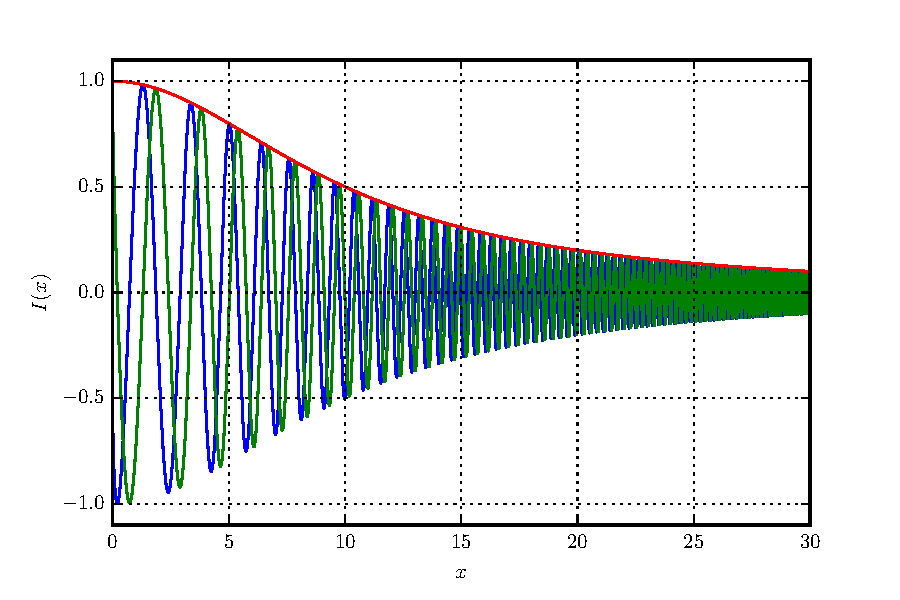
\includegraphics[width=\linewidth]{./fig/oscillatory_example_semiopen.pdf}
    \end{figure}
  \end{minipage}
  \begin{minipage}{0.49\linewidth}
    \begin{equation*}
      h_a(\tau) = \log(1 + \imath\tau)^2
    \end{equation*}
    \begin{figure}
      \centering
%       \includegraphics[width=0.6\linewidth]{./fig/nsd_path_semiopen_figure.pdf}
      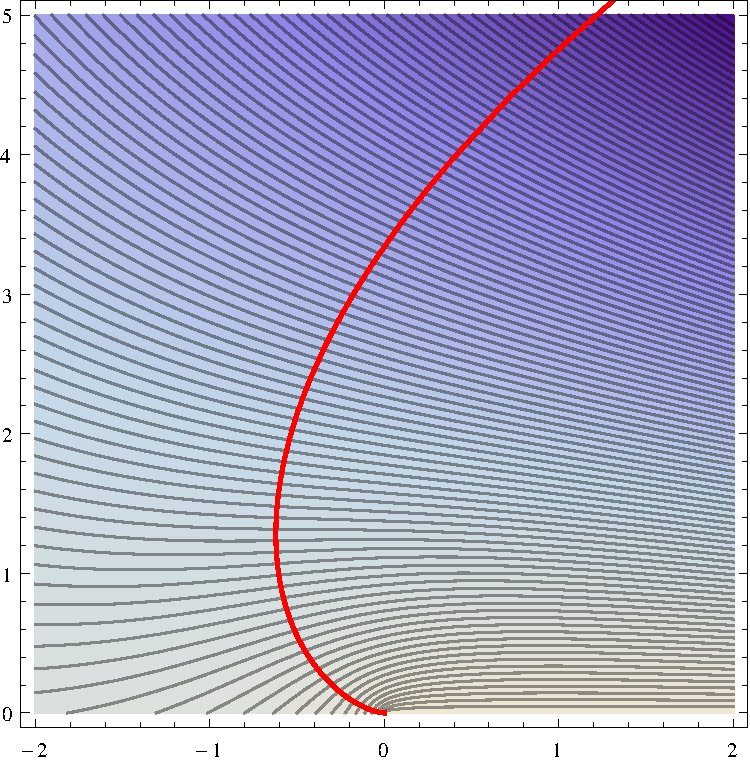
\includegraphics[width=0.6\linewidth]{./fig/oscillatory_example_semiopen_path.pdf}
    \end{figure}
    \scriptsize
    \begin{equation*}
      I = 200 e^{\imath\omega}
          \int_0^{\infty}
            \frac{\imath \log(1+\imath\tau) e^{-\omega\tau}}
                 {(1 + \imath\tau)\left(100+\log^4(1+\imath\tau)\right)}
          \di{\tau}
    \end{equation*}
  \end{minipage}
\end{frame}


\begin{frame}{Numerical Steepest Descent}{Literature}
  \nocite{nsd}{AH_cgq}
  \nocite{nsd}{HV_hoq}
  \nocite{nsd}{HV_cub}
  \nocite{nsd}{H_nsd_sii}
  \scriptsize
  \bibliographystyle{nsd}{abbrv}
  \bibliography{nsd}{nsd}{}
  \vspace{0.4cm}
  \footnoterule
  {\tiny The proof given by Majidian is wrong!}
\end{frame}


\section{Hagedorn Wavepackets}


\begin{frame}{Hagedorn Wavepackets}
  \begin{itemize}
    \item Time-dependent Schr\"odinger Equation (TDSE)
    \begin{equation*}
      \imath \varepsilon^2 \pdiff{\Psi}{t} = \left(-\frac{\varepsilon^4}{2}\Delta_x + V(\vec{x})\right) \Psi
    \end{equation*}
    \vspace{0.3cm}
    \item semiclassical scaling: $\varepsilon^2$ instead of $\hbar$
    \begin{itemize}
      \item $0.001 < \varepsilon < 0.1$
    \end{itemize}
  \end{itemize}
\end{frame}


\begin{frame}{Hagedorn Wavepackets}{Definition}
  \begin{itemize}
    \item Diagonalize quadratic Hamiltonian
      \begin{equation*}
        \mathcal{H} = \frac{1}{2} \left(\alpha p^2 + \beta (x p + p x) + \gamma x^2\right)
      \end{equation*}
    \item Position $x$ and momentum $p$
    \item Eigenvalues: $k + \frac{1}{2}$
    \item Eigenfunctions: $\phi_k, \quad k = 0, 1, 2, \ldots$
    \item Yields wavepackets $\phi_k(x)$
  \end{itemize}
\end{frame}


\begin{frame}{Hagedorn Wavepackets}{Explicit Representation in 1D}
  \begin{itemize}
    \item Explicit expression
    {\scriptsize
    \begin{align*}
      \phi_0(x) = (\pi\varepsilon^2)^{-\frac{1}{4}} Q^{-\frac{1}{2}}
                   \exp \left( \frac{\imath}{2\varepsilon^2} PQ\inv (x-q)^2 + \frac{\imath}{\varepsilon^2} p (x-q) \right)
    \end{align*}}
    \item Parametrized by $q(t), p(t) \in \mathbb{R}$ and $Q(t), P(t) \in \mathbb{C}$
    \item Raising and Lowering Operators
    \begin{align*}
      \phi_{k+1} = \frac{1}{\sqrt{k+1}} \mathcal{R} \phi_k
      \qquad
      \phi_{k-1} = \frac{1}{\sqrt{k}} \mathcal{L} \phi_k
    \end{align*}
    \item $\mathcal{L} \phi_0 \equiv 0$
    \item Orthonormal Basis of $L^2(\mathbb{R})$
  \end{itemize}
\end{frame}


\begin{frame}{Hagedorn Wavepackets}{Examples in 1D}
  \begin{figure}
    \centering
    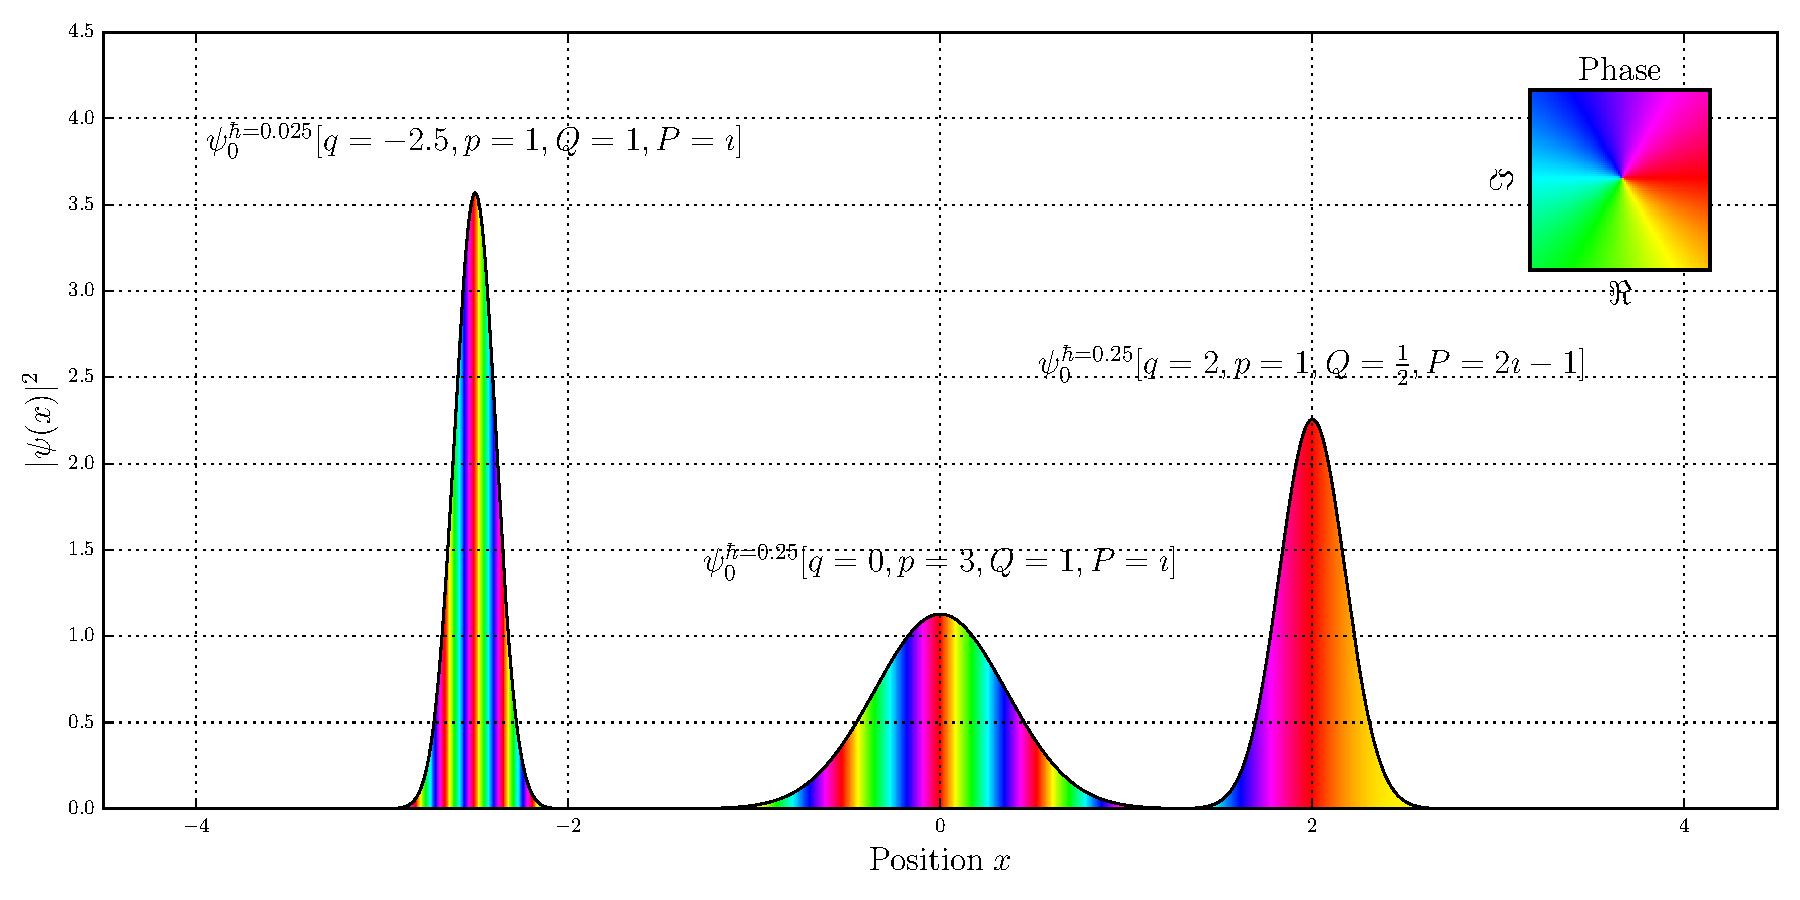
\includegraphics[width=\linewidth]{./fig/wavepackets.pdf}
  \end{figure}
\end{frame}


\begin{frame}{Hagedorn Wavepackets}{Explicit Representation in Higher Dimensions}
  \begin{itemize}
    \item Groundstate
    {\scriptsize
    \begin{align*}
      \phi_{\vec{0}}\left(\vec{x}\right)
      =
      (\pi\varepsilon^2)^{-\frac{D}{4}} (\det\mat{Q})^{-\frac{1}{2}}
      \exp \left( \frac{\imath}{2\varepsilon^2}
      \dotp{(\vec{x}-\vec{q})}{\mat{P}\mat{Q}\inv(\vec{x}-\vec{q})}
      + \frac{\imath}{\varepsilon^2} \dotp{\vec{p}}{(\vec{x}-\vec{q})}
      \right)
    \end{align*}}
    \item Parameters $\vec{q}(t), \vec{p}(t) \in \mathbb{R}^D$ and $\mat{Q}(t), \mat{P}(t) \in \mathbb{C}^{D \times D}$
    \begin{itemize}
      \item Parameter set $\Pi \assign \{\vec{q}, \vec{p}, \mat{Q}, \mat{P}\}$
    \end{itemize}
%     \item Compatibility
%     \begin{align*}
%       \mat{Q}\H \mat{P} - \mat{P}\H \mat{Q} = 2\imath \id
%       \qquad
%       \mat{P}\T \mat{Q} - \mat{Q}\T \mat{P} = \mat{0}
%     \end{align*}
%    \item $\mathcal{R}, \mathcal{L}$ much more complicated
    \vspace{0.2cm}
    \item Multi-index $\vec{k} \in \mathbb{N}_0^D$
    \item Higher states by raising and lowering operators $\mathcal{R}$, $\mathcal{L}$
    \item Orthonormal Basis of $L^2(\mathbb{R}^D)$
  \end{itemize}
\end{frame}


\begin{frame}{Hagedorn Wavepackets}{Example in 2D}
  \vspace{-0.4cm}
  \scriptsize
  \begin{equation*}
    \phi_{\vec{k}}[\Pi](\vec{x}) \quad\quad \vec{k} = (1,3) \quad \varepsilon = \frac{1}{10}
  \end{equation*}
  \vspace{-0.4cm}
  \begin{figure}[h!]
    \centering
    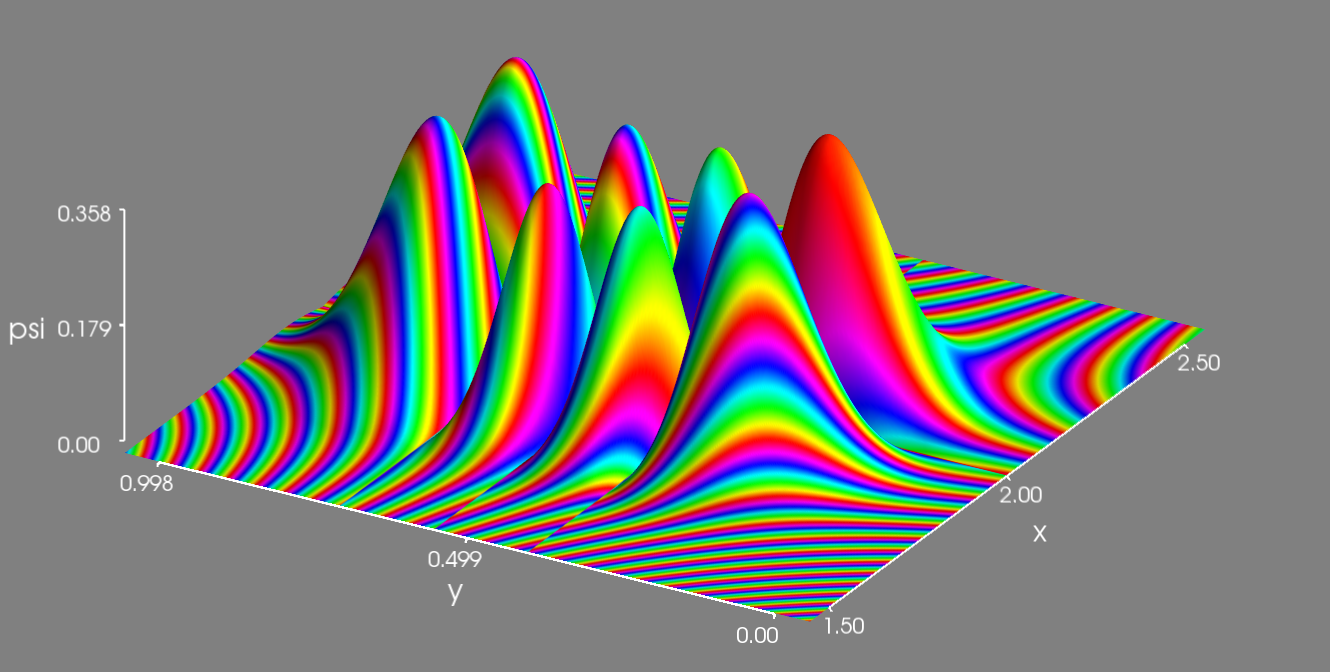
\includegraphics[width=0.8\linewidth]{./fig/wavepackets_2d.png}
  \end{figure}
    \scriptsize
  \begin{equation*}
    \vec{q} =
    \begin{pmatrix}
      2 \\ \sqrt{3\varepsilon}
    \end{pmatrix}
    \quad
    \vec{p} =
    \begin{pmatrix}
      -\frac{2}{5} \\ \sqrt{\frac{4\varepsilon}{12}}
    \end{pmatrix}
    \quad
    \mat{Q} =
    \begin{pmatrix}
      1 & 0 \\
      0 & \frac{1}{\sqrt{\frac{4}{5}}}
    \end{pmatrix}
    \quad
    \mat{P} =
    \begin{pmatrix}
      -2+\imath & -3 \\
      -3\sqrt{\frac{4}{5}} & \imath\sqrt{\frac{4}{5}}
    \end{pmatrix}
  \end{equation*}
\end{frame}


\subsection{Overlap integrals}


\begin{frame}{Hagedorn Wavepackets}{}
  \begin{itemize}
    \item Overlap integrals
    \begin{equation*}
      I
      = \Braket{\phi_\vec{k}[\Pi] | \phi_\vec{l}[\Pi^\prime]}
      \assign \idotsint_{\mathbb{R}^D} \conj{\phi_\vec{k}[\Pi](\vec{x})}
                                          \, \phi_\vec{l}[\Pi^\prime](\vec{x}) \di{\vec{x}}
    \end{equation*}
    \item Parameter sets: $\Pi$ and $\Pi^\prime$
    \item Highly oscillatory
    \begin{itemize}
      \item similar position: $\vec{q} \approx \vec{q}^\prime$
      \item opposite momentum: $\vec{p} \approx -\vec{p}^\prime$
      \item small $\varepsilon$
    \end{itemize}
  \end{itemize}
\end{frame}


\begin{frame}{Hagedorn Wavepackets}{Two Wavepackets}
  \begin{figure}
    \centering
    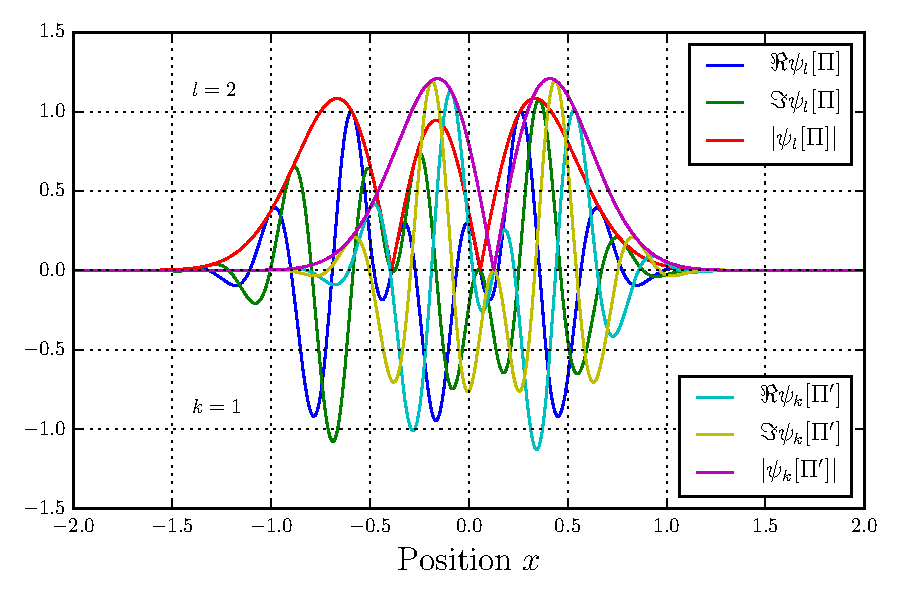
\includegraphics[width=0.8\linewidth]{./fig/overlap_wavepackets.pdf}
  \end{figure}
\end{frame}


\begin{frame}{Hagedorn Wavepackets}{The Integrand}
  \begin{figure}
    \centering
    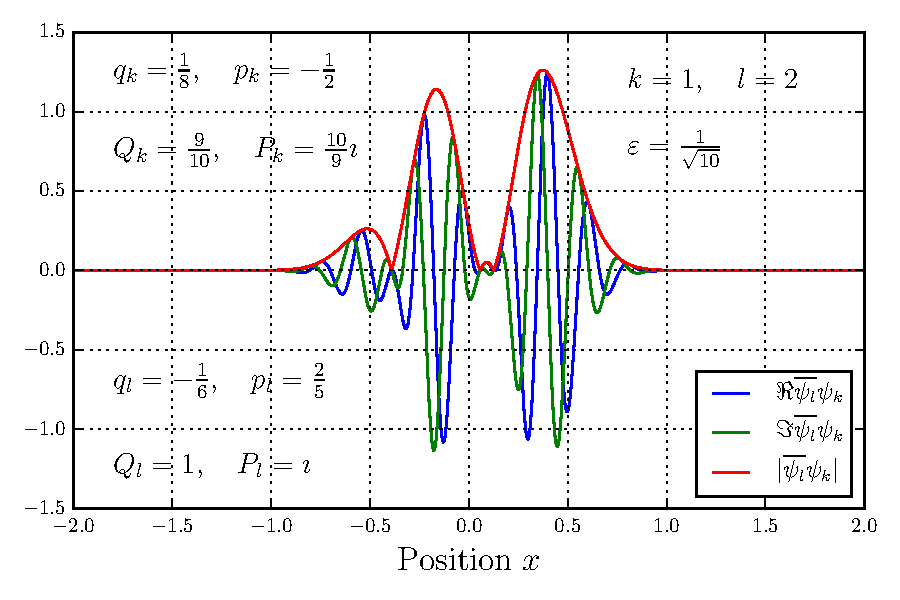
\includegraphics[width=0.8\linewidth]{./fig/overlap_integrand.pdf}
  \end{figure}
\end{frame}


\begin{frame}{Hagedorn Wavepackets}{Literature}
  \nocite{hawp}{B_master_thesis}
  \nocite{hawp}{H_ladder_operators}
  \scriptsize
  \bibliographystyle{hawp}{abbrv}
  \bibliography{hawp}{mt,../../references/own}{}
\end{frame}


\section{Steepest Descent for Wavepackets}


\begin{frame}{Steepest Descent for Wavepackets}{Wavepackets}
  \begin{itemize}
    \item Wavepackets of the form:
    \begin{equation*}
      \phi(\vec{x}) \sim p\left(\vec{x}\right)\exp\left(\frac{\imath}{\varepsilon^2} g\left(\vec{x}\right)\right)
    \end{equation*}
    \item Oscillator term:
    \begin{equation*}
      g\left(\vec{x}\right)
      \assign
      \frac{1}{2} \dotp{\vec{x}-\vec{q}}{\mat{P}\mat{Q}\inv \left(\vec{x}-\vec{q}\right)}
      +
      \dotp{\vec{p}}{\vec{x}-\vec{q}}
    \end{equation*}
    \item Frequency $\omega = \frac{1}{\varepsilon^2}$
  \end{itemize}
\end{frame}


\begin{frame}{Steepest Descent for Wavepackets}{Overlap Integrals}
  \begin{itemize}
    \item Integrals look like
    \begin{equation*}
      \dotp{\phi_k}{\phi_l} =
      \int_{-\infty}^{\infty}
        \conj{p_k(\vec{x})} p_l(\vec{x})
        \exp\left(\frac{\imath}{\varepsilon^2}\left(-\conj{g_k(\vec{x})} + g_l(\vec{x})\right)\right)
      \mathrm{d}\vec{x}
    \end{equation*}
    \item Combine oscillators $-\conj{g_k(\vec{x})} + g_l(\vec{x})$ into $g(\vec{x})$
  \end{itemize}
\end{frame}


\begin{frame}{Steepest Descent for Wavepackets}{Combined Oscillator}
  \begin{itemize}
    \item We can find
    \begin{equation*}
      g(\vec{x}) = \vec{x}\H \mat{A} \vec{x} + \vec{b}\T \vec{x} + c
    \end{equation*}
    \item where
    \begin{equation*}
      \mat{A} = \frac{1}{2} \left(\mat{P_l}\mat{Q_l}\inv - (\mat{P_k}\mat{Q_k}\inv)\H \right)
    \end{equation*}
    \item General quadratic form
    \item Properties of $A$
    \begin{itemize}
      \item $\mat{A}$ \cemph{not} Hermitian
      \item $\Re \mat{A}$ and $\Im \mat{A}$ symmetric
      \\[0.1cm]$\Rightarrow$ Need new, special techniques
    \end{itemize}
  \end{itemize}
\end{frame}


\begin{frame}{Steepest Descent for Wavepackets}{Transformation of the Oscillator}
  \begin{itemize}
    \item Goal: Decoupling the paths
    \vspace{0.3cm}
    \item Remove linear Term $\vec{b}\T \vec{x}$
    \begin{itemize}
      \item Multivariate completion of the square
      \item $g(x^\prime) = x^\prime\H \mat{A} x^\prime + c$
    \end{itemize}
    \item Diagonalization of $\mat{A}$
    \begin{itemize}
      \item Optimal, \cemph{not} possible via unitary matrices ($\mat{A}$ not Hermitian)
    \end{itemize}
    \item Upper-triangular form
    \begin{itemize}
      \item Schur Decomposition: $\mat{A} = \mat{U}\H \mat{T} \mat{U}$
      \item $g(x^{\prime\prime}) = x^{\prime\prime}\H \mat{T} x^{\prime\prime} + c^{\prime}$
    \end{itemize}
%     \item Transformations have unit Jacobi determinants
  \end{itemize}
\end{frame}


\begin{frame}{Steepest Descent for Wavepackets}{Oscillator Decomposition}
  \begin{itemize}
    \item Decompose $g(\vec{x}) = \vec{x}\H\mat{T}\vec{x}$
    \begin{equation*}
      g\left(x_1, \ldots, x_N\right) = \sum_{i=1}^N g_i(x_i, \ldots, x_N)
    \end{equation*}
    \item where
    \begin{equation*}
      g_i\left(x_i, x_{i+1}, \ldots, x_N\right)
      \assign t_{i,i} x_i^2 + \sum_{j=i+1}^{N} t_{i,j} x_i x_j
    \end{equation*}
    \item Quadratic in $x_{i}$
    \item Rows of $\mat{T}$
  \end{itemize}
\end{frame}


\begin{frame}{Steepest Descent for Wavepackets}{Stationary Points}
  \begin{itemize}
    \item Compute stationary points
    \begin{equation*}
      \dot{g}_i \assign \pdiff{g_i}{x_i} \stackrel{!}{=} 0
    \end{equation*}
    \item Find
    \begin{equation*}
      x_i^{*}\left(x_{i+1}, \ldots, x_N\right)
      = - \frac{ \sum_{j=i+1}^{N} t_{i,j} x_j }{ 2 t_{i,i} }
    \end{equation*}
    \item Depends on $x_{i+1}, \ldots, x_N$
  \end{itemize}
\end{frame}


\begin{frame}{Steepest Descent for Wavepackets}{Path Equations}
  \begin{itemize}
    \item For each oscillator $g_i$
    \begin{equation*}
      g_i\left(h_i\left(p_i,\ldots\right), \ldots\right)
      = g_i\left(x_i^{*}(\ldots), \ldots\right) + \imath p_i
    \end{equation*}
    \item Each $\ldots$ is $x_{i+1}, \ldots, x_{N}$
    \item Simple quadratic equations
    \item Paths:
    \begin{equation*}
      h_i^{\pm}(p_i)
      =
      \pm \sqrt{\frac{\imath p_i}{t_{i,i}}}
      -\frac{1}{2 t_{i,i}} \sum_{j=i+1}^{N} t_{i,j} x_j
    \end{equation*}
    \item Path derivatives:
    \begin{equation*}
      \dot{h}_i^{\pm}(p_i) = \pdiff{h_i\left(p_i\right)}{p_i}
      = \pm \frac{\sqrt{\imath}}{2 \sqrt{t_{i,i}}\sqrt{p_i}}
    \end{equation*}
  \end{itemize}
\end{frame}


\begin{frame}{Steepest Descent for Wavepackets}{Nested Structure of Oscillatory Integrals}
  \begin{itemize}
    \item Start with inner-most integrand
    \begin{equation*}
      i_1\left(x_1,\ldots,x_N\right) \assign f\left(\vec{x}\right) \exp\left(i\omega g_1\left(x_1,\ldots,x_N\right)\right)
    \end{equation*}
    \item Compute integral
    \begin{equation*}
      I_1\left(x_2,\ldots,x_N\right) = \int_{-\infty}^\infty i_1\left(x_1,\ldots,x_N\right) \mathrm{d}x_1
    \end{equation*}
    \item Iterate until \ldots
    \begin{equation*}
      i_N\left(x_N\right) \assign I_{N-1}\left(x_N\right) \exp\left(i\omega g_N\left(x_N\right)\right)
    \end{equation*}
    \item outer-most integral
    \begin{equation*}
      I = I_N\left(\right) = \int_{-\infty}^\infty i_N\left(x_N\right) \mathrm{d}x_N
    \end{equation*}
  \end{itemize}
\end{frame}


\begin{frame}{Steepest Descent for Wavepackets}{Transformation of the Integrals}
  \begin{itemize}
    \item For each oscillatory part
    \begin{equation*}
      \exp\left(i\omega g_i\left(x_i,\ldots,x_N\right)\right)
      =
      C
      %\exp\left(i\omega k_i\left(x_{i+1},\ldots,x_N\right)\right)
      \exp\left(- \omega p_i\right)
    \end{equation*}
    \item Variable transformation by paths
    \begin{equation*}
        I_i^{\pm}[h_i^{\pm}] =
        C
        %\exp\left(i\omega k_i\right)
        \int_0^\infty
          i_i\left(h_i^{\pm}\left(p_i\right)\right)
          \dot{h}_i^{\pm}\left(p_i\right)
          \exp\left(- \omega p_i\right)
        \mathrm{d}p_i
    \end{equation*}
    \item Singular for $p_i \rightarrow 0$
    \item Substitute $q_i \assign \sqrt{p_i}$
    \begin{equation*}
        I_i^{\pm}[h_i^{\pm}] =
        C
        %\exp\left(i\omega k_i\right)
        \int_0^\infty
          i_i\left(h_i^{\pm}\right)
          \ldots
          \exp\left(- \omega q_i^2\right)
        \mathrm{d}q_i
    \end{equation*}
  \end{itemize}
\end{frame}


\begin{frame}{Steepest Descent for Wavepackets}{Gluing Paths}
  \begin{itemize}
    \item Two times half of a Gaussian integral
    \item Glue paths:
    \begin{equation*}
      I_i[h_i] =
      I_i^{+}[h_i^{+}]
      -
      I_i^{-}[h_i^{-}]
    \end{equation*}
    \item Transform $h_i^{-}$ into $h_i^{+}$ by $\tau_i \assign -q_i$
    \item Full Gaussian Integral
    \begin{equation*}
      I_i\left(x_{i+1},\ldots,x_N\right) =
      C
      \int_{-\infty}^\infty
        i_i\left(h_i\left(\tau_i\right)\right)
        \ldots
        \exp\left(- \omega \tau_i^2\right)
      \mathrm{d}\tau_i
    \end{equation*}
  \end{itemize}
\end{frame}


\begin{frame}{Steepest Descent for Wavepackets}{Final Quadrature}
  \begin{itemize}
    \item Resolved nested integral
    \begin{equation*}
      I = \int_{-\infty}^\infty \cdots \int_{-\infty}^\infty
          f\left(\vec{h}(\vec{\tau})\right)
          \prod_{i=1}^N C_i
                        \exp\left(-\omega \tau_i^2\right)
          \mathrm{d}\tau_1 \cdots \mathrm{d}\tau_N
    \end{equation*}
    \item Apply Gauss-Hermite Quadrature $Q \approx I$
    \begin{equation*}
      Q =
      \prod_{j=1}^N
      C_j
      \sum_{k_1}^n \cdots \sum_{k_N}^n
      f\left(h_1\left(x_{k_1}\right),
           \ldots,
           h_N\left(x_{k_N}\right)
    \right)
    \prod_{i=1}^N w_{k_i}
    \end{equation*}
  \end{itemize}
\end{frame}


\begin{frame}{Steepest Descent for Wavepackets}{Literature}
  \nocite{sdwp}{BG_nsd}
  \scriptsize
  \bibliographystyle{sdwp}{abbrv}
  \bibliography{sdwp}{../../references/own}{}
\end{frame}


\section{Sparse Quadrature Schemes}


\begin{frame}{Sparse Quadrature Schemes}
  \begin{itemize}
  \item Problem:
    \begin{itemize}
    \item full tensor-product quadrature
    \begin{itemize}
      \item with less nodes per direction
    \end{itemize}
    \end{itemize}
  \end{itemize}
  \vspace{0.5cm}
  \begin{itemize}
  \item Solution:
    \begin{itemize}
    \item Sparse grid schemes
    \begin{itemize}
      \item Smolyak rule
    \end{itemize}
    \end{itemize}
  \end{itemize}
\end{frame}


\begin{frame}{Sparse Quadrature Schemes}{Smolyak Construction}
  \begin{itemize}
    \item Smolyak construction:
    \begin{equation*}
      S_{D,k} \assign \sum_{q=k-D}^{k-1} (-1)^{k-1-q} \binom{D-1}{k-1-q}
                      \sum_{\substack{\vec{l} \in \mathbb{N}^D \\
                                      \|\vec{l}\|_1 = D+q}}
                        \left(Q_{l_1} \otimes \cdots \otimes Q_{l_D}\right)
    \end{equation*}
    \item Sum of many (smaller) tensor products
  \end{itemize}
\end{frame}


\begin{frame}{Sparse Quadrature Schemes}
  Construction with Gauss-Hermite rules
  \begin{figure}
    \centering
    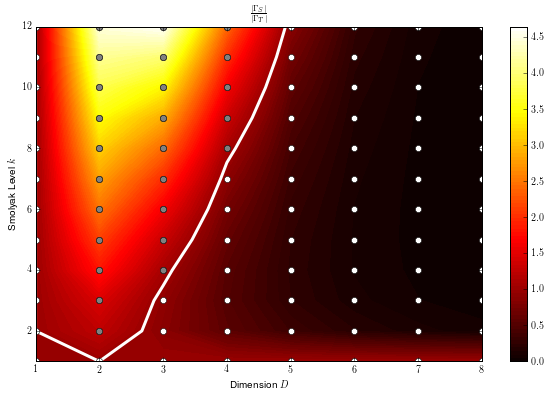
\includegraphics[width=0.8\linewidth]{./fig/smolyak_gauss_ratiomap.png}
  \end{figure}
\end{frame}


\begin{frame}{Sparse Quadrature Schemes}{Smolyak Construction Issues}
  \begin{itemize}
    \item Problem:
    \begin{itemize}
      \item Gauss-Hermite points not nested
      \begin{itemize}
        \item more points than full tensorproduct!
      \end{itemize}
    \end{itemize}
    \vspace{0.5cm}
    \item Solution:
    \begin{itemize}
      \item Search rules with nested nodes
      \item For interval $(-\infty, \infty)$ with weight $\exp(-x^2)$
      \begin{itemize}
        \item Iterative \cemph{Kronrod} extensions
        \item \cemph{Genz-Keister} rules
      \end{itemize}
    \end{itemize}
  \end{itemize}
\end{frame}


\begin{frame}{Sparse Quadrature Schemes}{Genz-Keister Nodes}
  \begin{figure}
    \centering
    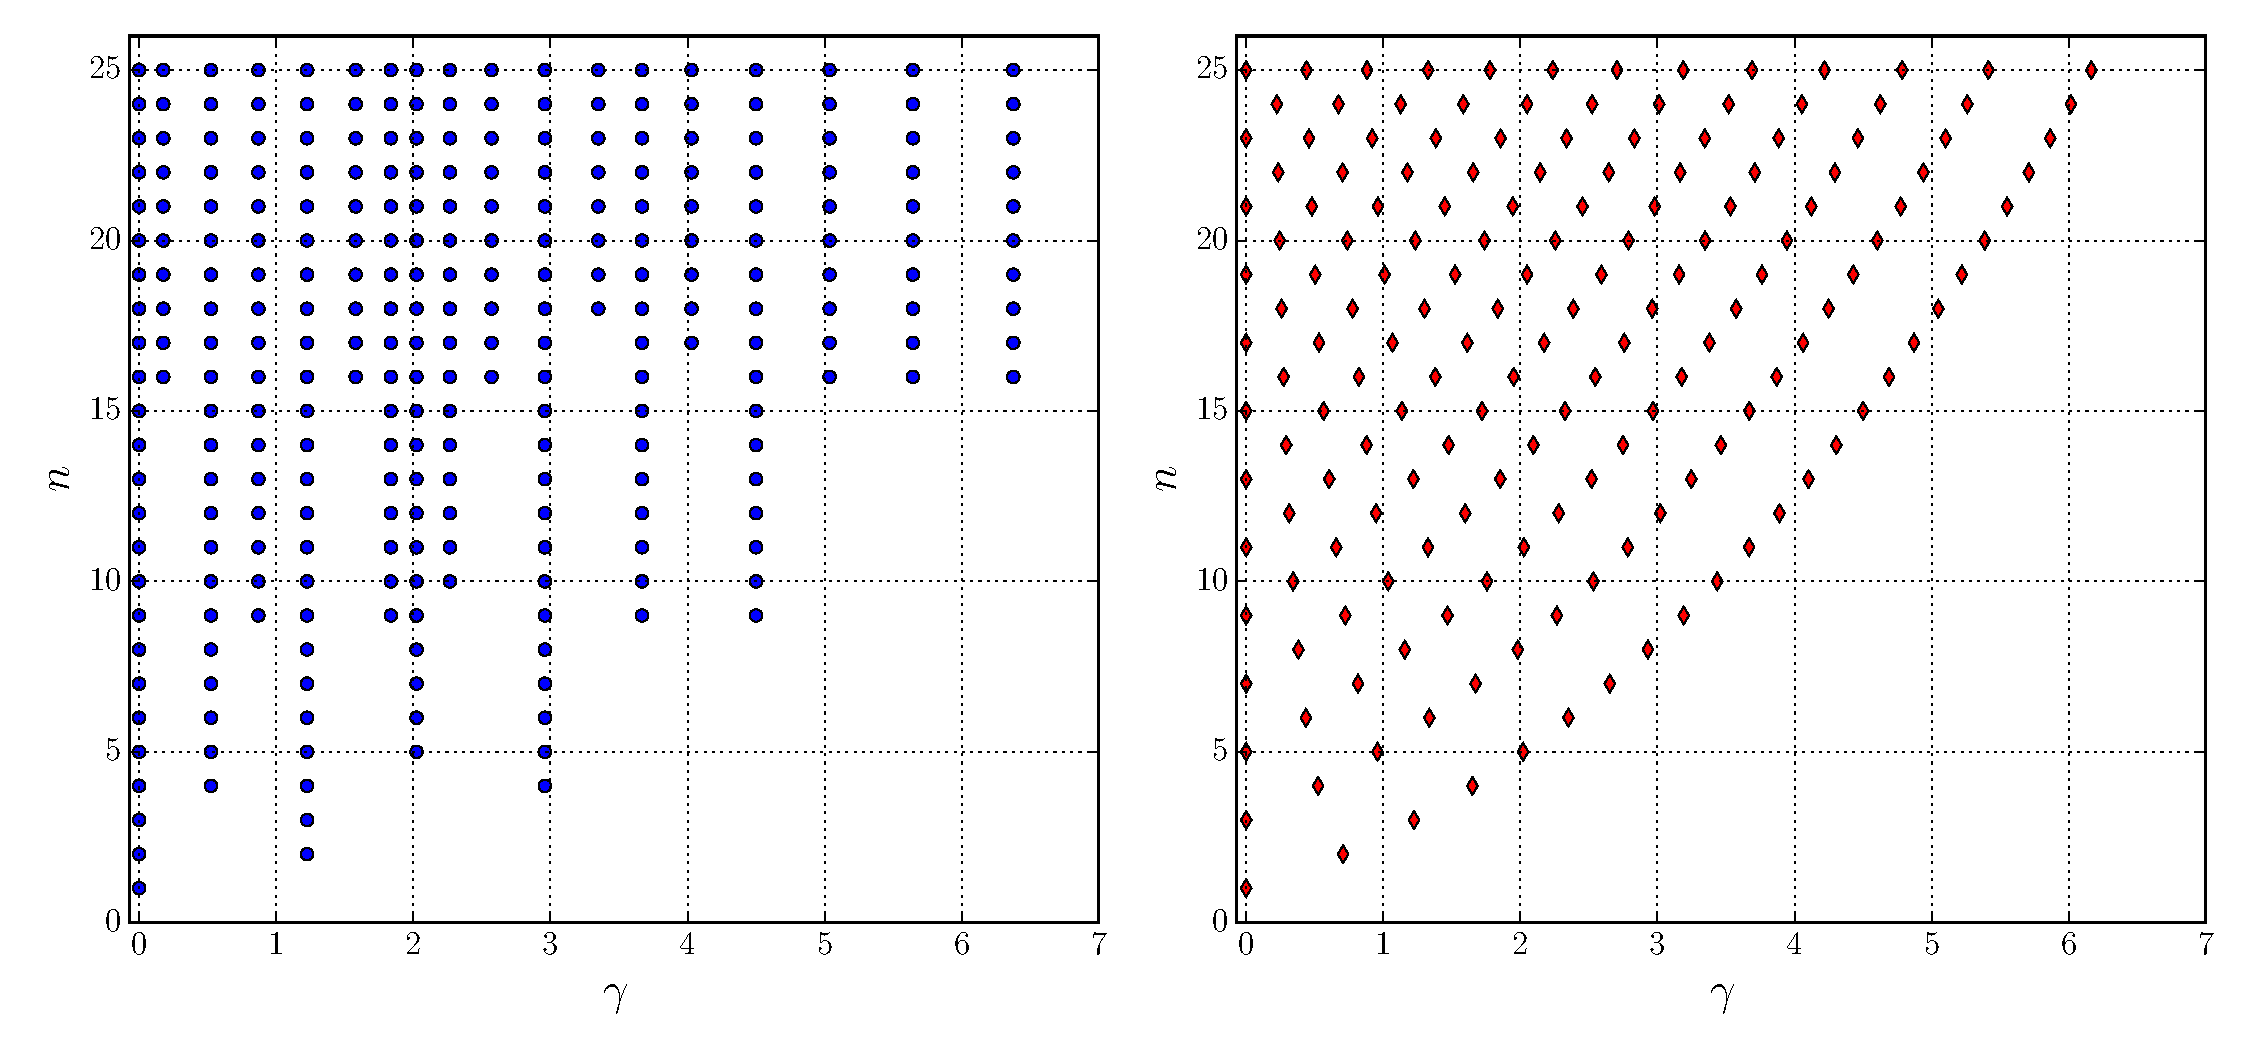
\includegraphics[width=\textwidth]{./fig/genz_keister_nodes.pdf}
  \end{figure}
\end{frame}


\begin{frame}{Sparse Quadrature Schemes}
  Construction with Genz-Keister nested rules
  \begin{figure}
    \centering
    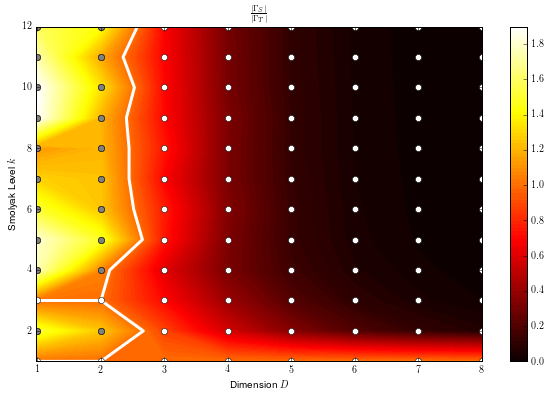
\includegraphics[width=0.8\linewidth]{./fig/smolyak_genzkeister_ratiomap.png}
  \end{figure}
\end{frame}


\begin{frame}{Final Solution for computing overlap Integrals}
  \begin{itemize}
    \item Chain of Transformators
    \begin{itemize}
      \item Steepest Descent: \cemph{remove oscillations}
      \item Sparse Grid: \cemph{lessen curse of dimensionality}
      \item Genz-Keister rules: \cemph{make nodes nested}
    \end{itemize}
  \end{itemize}
  \begin{figure}
    \centering
    \includegraphics[width=\linewidth]{./fig/diagram4.pdf}
  \end{figure}
\end{frame}


\begin{frame}{Sparse Quadrature Schemes}{Literature}
  \nocite{sqs}{genz_keister}
  \nocite{sqs}{mehrotra-papp}
  \nocite{sqs}{B_kes}
  \scriptsize
  \bibliographystyle{sqs}{abbrv}
  \bibliography{sqs}{sparse,kes,../../references/own}{}
\end{frame}


\section{Numerical Experiments and Examples}

% Harmonic Channel
% Harmonic Tube

\begin{frame}{Numerical Experiments}{Convergence}
  \begin{figure}
    \centering
    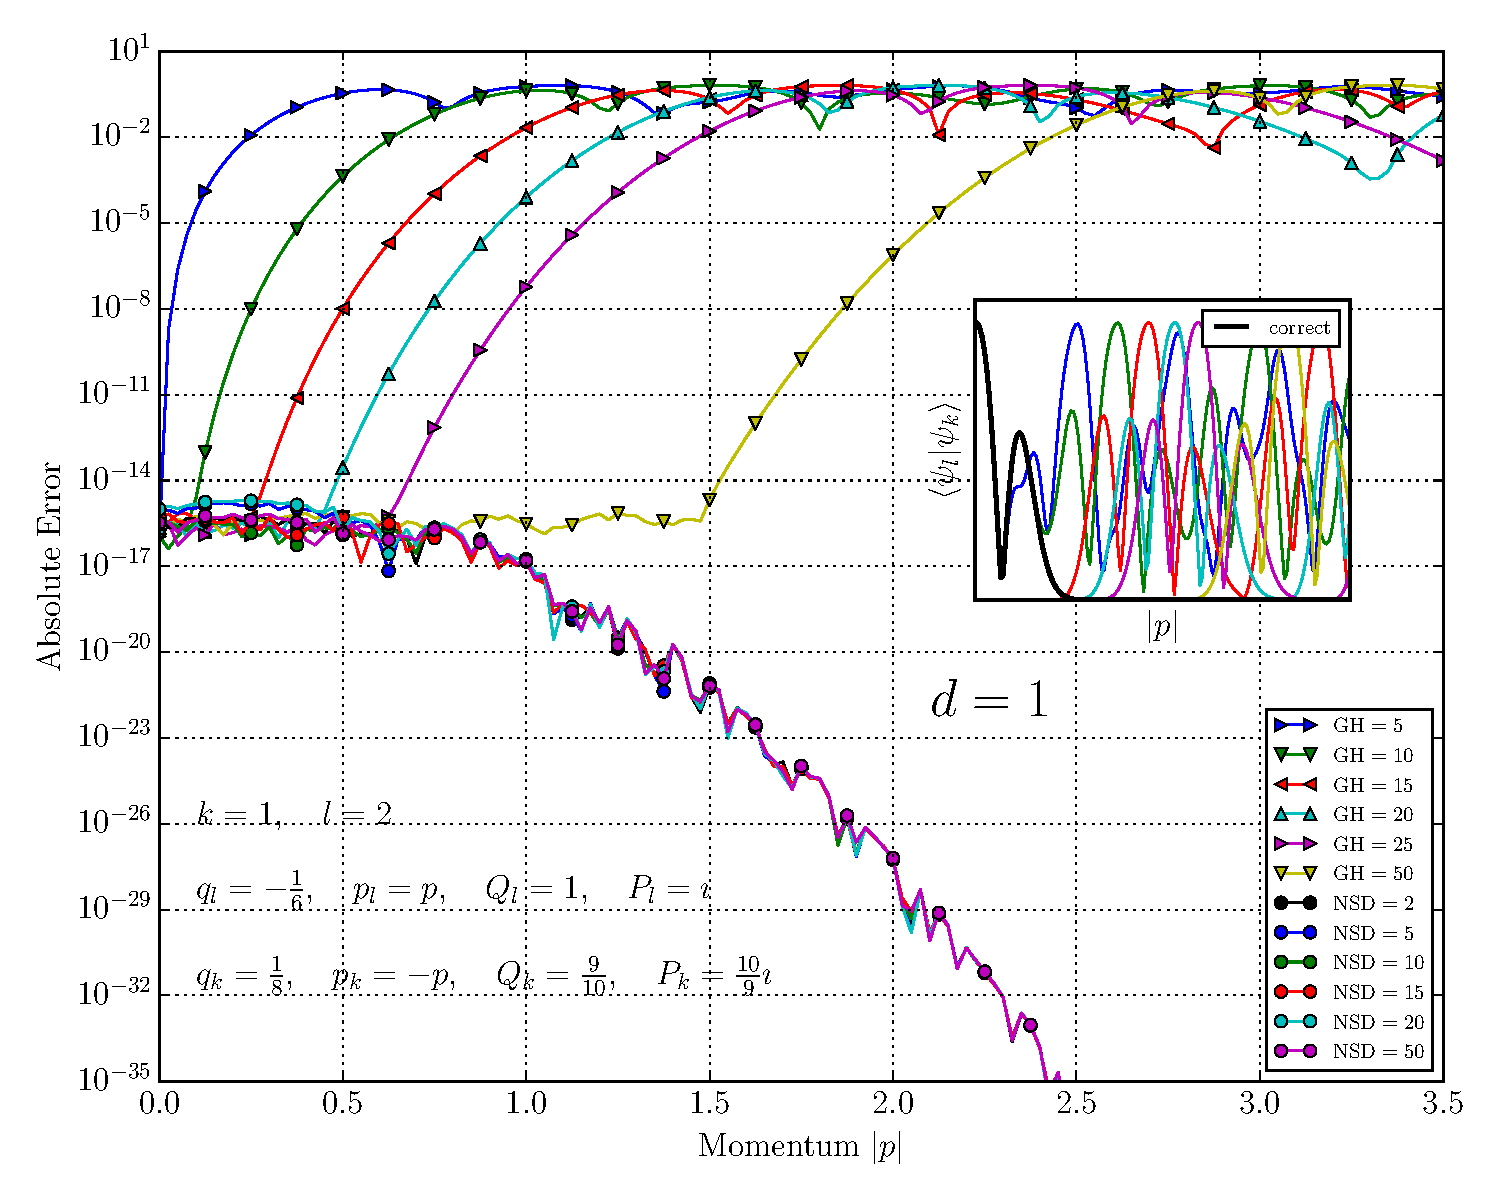
\includegraphics[width=0.65\linewidth]{./fig/conv_momentum.pdf}
  \end{figure}
  \scriptsize
  Gauss-Hermite is wrong, Steepest Descent Transformation is perfect
\end{frame}


\begin{frame}{Numerical Experiments}{Convergence}
  \begin{figure}
    \centering
    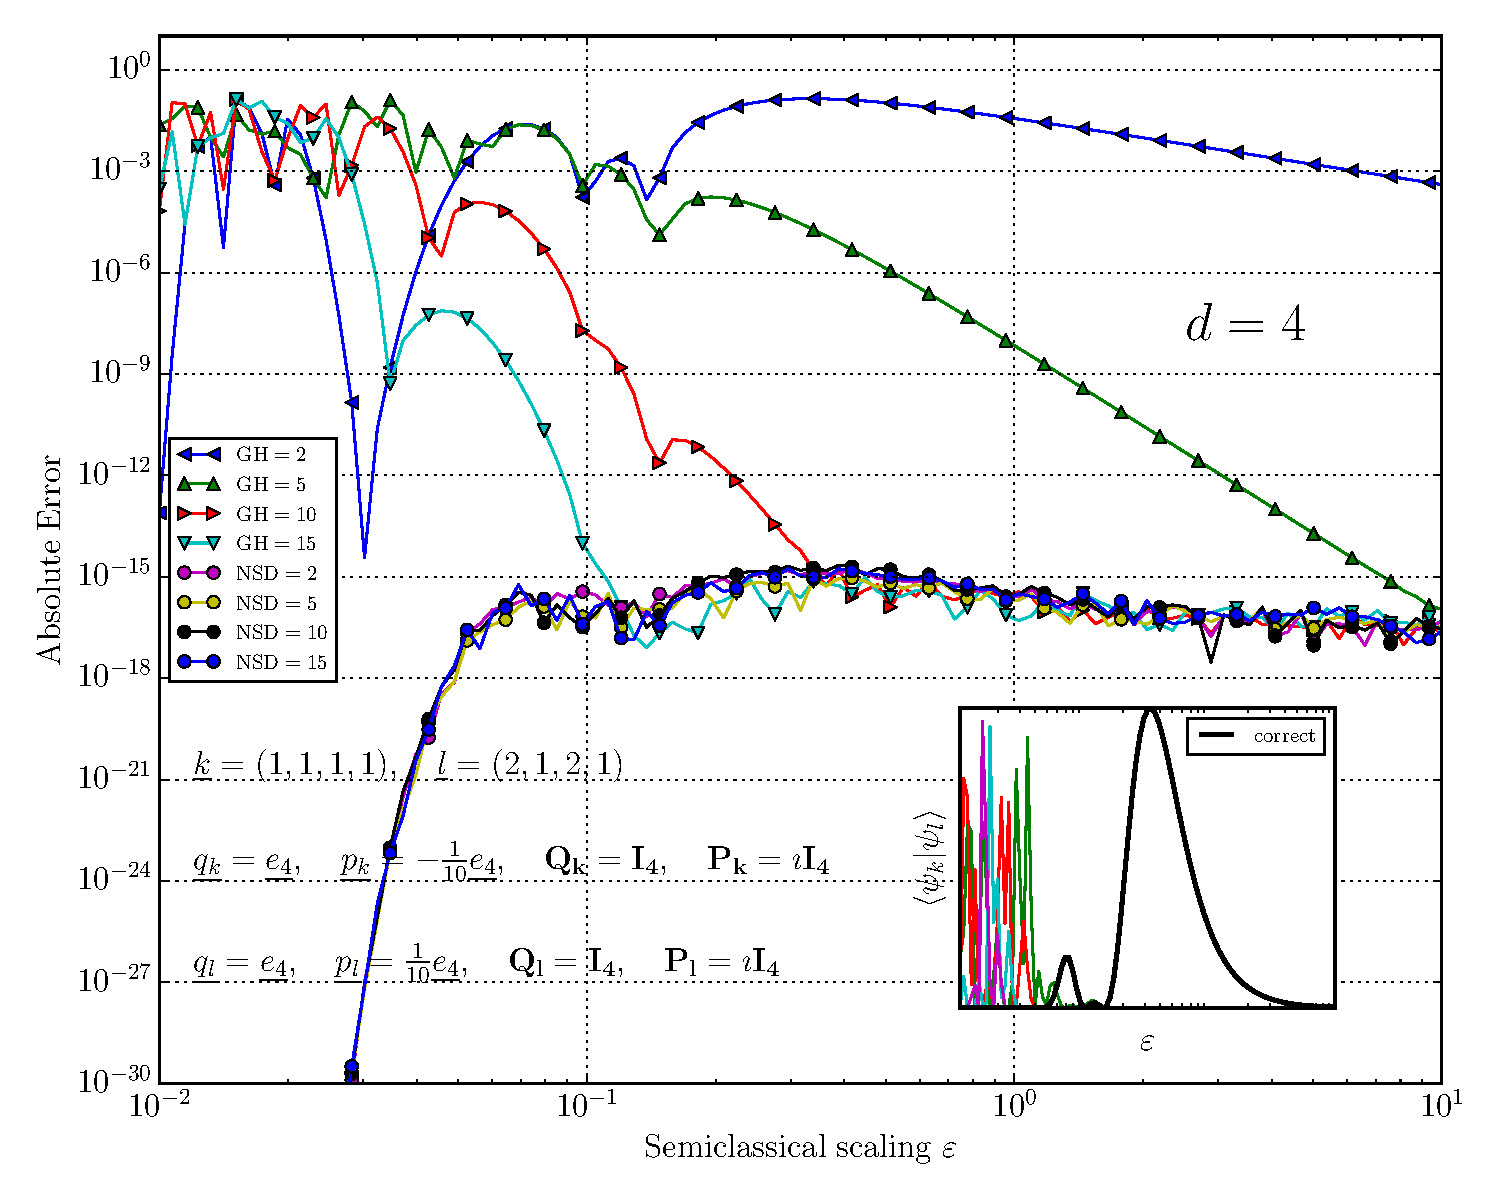
\includegraphics[width=0.7\linewidth]{./fig/conv_eps.pdf}
  \end{figure}
  \scriptsize
  Gauss-Hermite is wrong, Steepest Descent Transformation is perfect
\end{frame}


\begin{frame}{Real-world Example \ce{Hg2}}
  \begin{itemize}
    \item Compute autocorrelation $|A(t)|$ by improved integrator
  \end{itemize}
  \vspace{0.2cm}
  \begin{equation*}
    A(t) \assign \Braket{\Psi_0 | \Psi_t}
         = \idotsint_{\mathbb{R}^D} \conj{\Psi_0(\vec{x})} \Psi_t(\vec{x}) \di{\vec{x}}
  \end{equation*}
  \begin{figure}
    \centering
    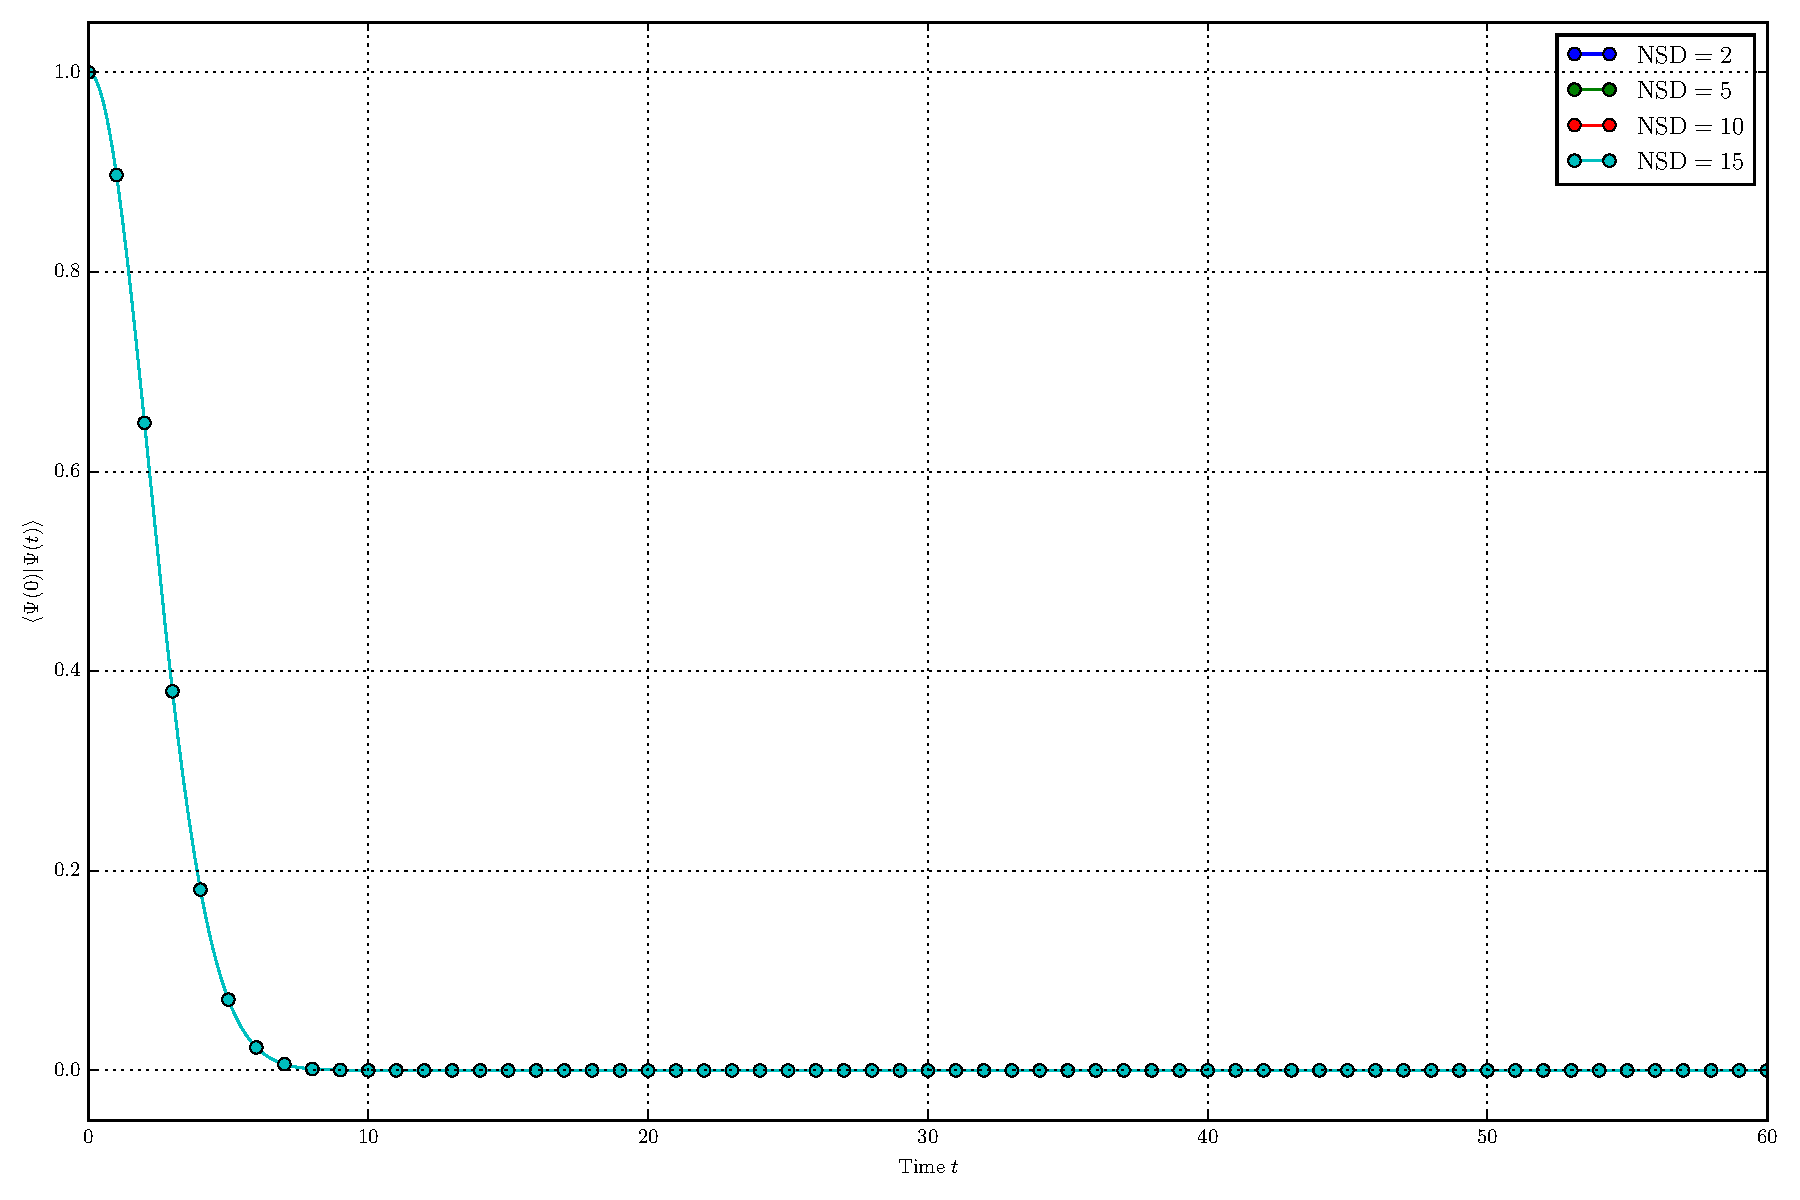
\includegraphics[width=0.7\linewidth]{./fig/ac_mercurial_morse_nsd.pdf}
  \end{figure}
\end{frame}


\section{Future Work and Open Topics}


\begin{frame}{Future Work and Open Topics}
  \begin{itemize}
    \item Proof steepest descent technique for (semi-)infinite intervals
    \item Other integrals like $\braket{\phi|V|\phi}$
    \begin{itemize}
      \item Potentials with non-polynomial or exponential parts
    \end{itemize}
    \item Non-classical Smolyak constructions
    \begin{itemize}
      \item Hyperbolic cut sections
      \item Adaptive versions
    \end{itemize}
    \item Proof (non-)existence of higher Kronrod Extensions
    \item Implement much larger Genz-Keister rules
  \end{itemize}
\end{frame}


\section{End}


\begin{frame}{Thanks for your Attention}
  \begin{center}
    {\Huge{Questions?}}
  \end{center}
\end{frame}

\end{document}
